\section{Analiza wyników dla datasetu \textbf{BuzzFeed}}
\label{subsec:buzzfeed_analysis}

W tej sekcji przedstawiono wyniki dla datasetu \textbf{BuzzFeed} w trybach: \textbf{klasycznym}, \textbf{few-shot} oraz \textbf{one-shot}. Analiza obejmuje kluczowe metryki (Accuracy, F1-Score, ROC-AUC) dla embeddingów BERT, RoBERTa i SBERT, zwięźle omówione w kontekście wykresów. Dla metod autorskich (\texttt{Metoda17}--\texttt{Metoda20}) podano przyczyny wyników. Wnioski zebrano w sekcji podsumowującej.

\subsection{Wyniki w trybie klasycznym}

\subsubsection{Accuracy}
Wykresy Accuracy (\ref{fig:buzzfeed_classic_accuracy}) pokazują, że dla BERT \texttt{Metoda12-catboost}, \texttt{Metoda12-rf} i \texttt{Metoda19} osiągnęły ~0.6, a \texttt{Metoda18} najniższe (~0.38). Dla RoBERTa \texttt{Metoda10} i \texttt{Metoda12-catboost} osiągnęły ~0.68, a \texttt{Metoda1-2}, \texttt{Metoda17}, \texttt{Metoda19} ~0.49. Dla SBERT \texttt{Metoda13} i \texttt{Metoda12-catboost} miały ~0.73, a \texttt{Metoda1-3}, \texttt{Metoda3}, \texttt{Metoda4} ~0.49. \texttt{Metoda17} (VotingClassifier) zawodzi dla RoBERTa z powodu niedopasowania hiperparametrów, \texttt{Metoda18} (stacking) jest słaba dla BERT z powodu prostej architektury, \texttt{Metoda19} (stacking) osiąga wysokie wyniki dla BERT/SBERT dzięki zoptymalizowanemu łączeniu modeli, a \texttt{Metoda20} jest średnia z powodu braku balansowania klas.

\begin{figure}[H]
	\centering
	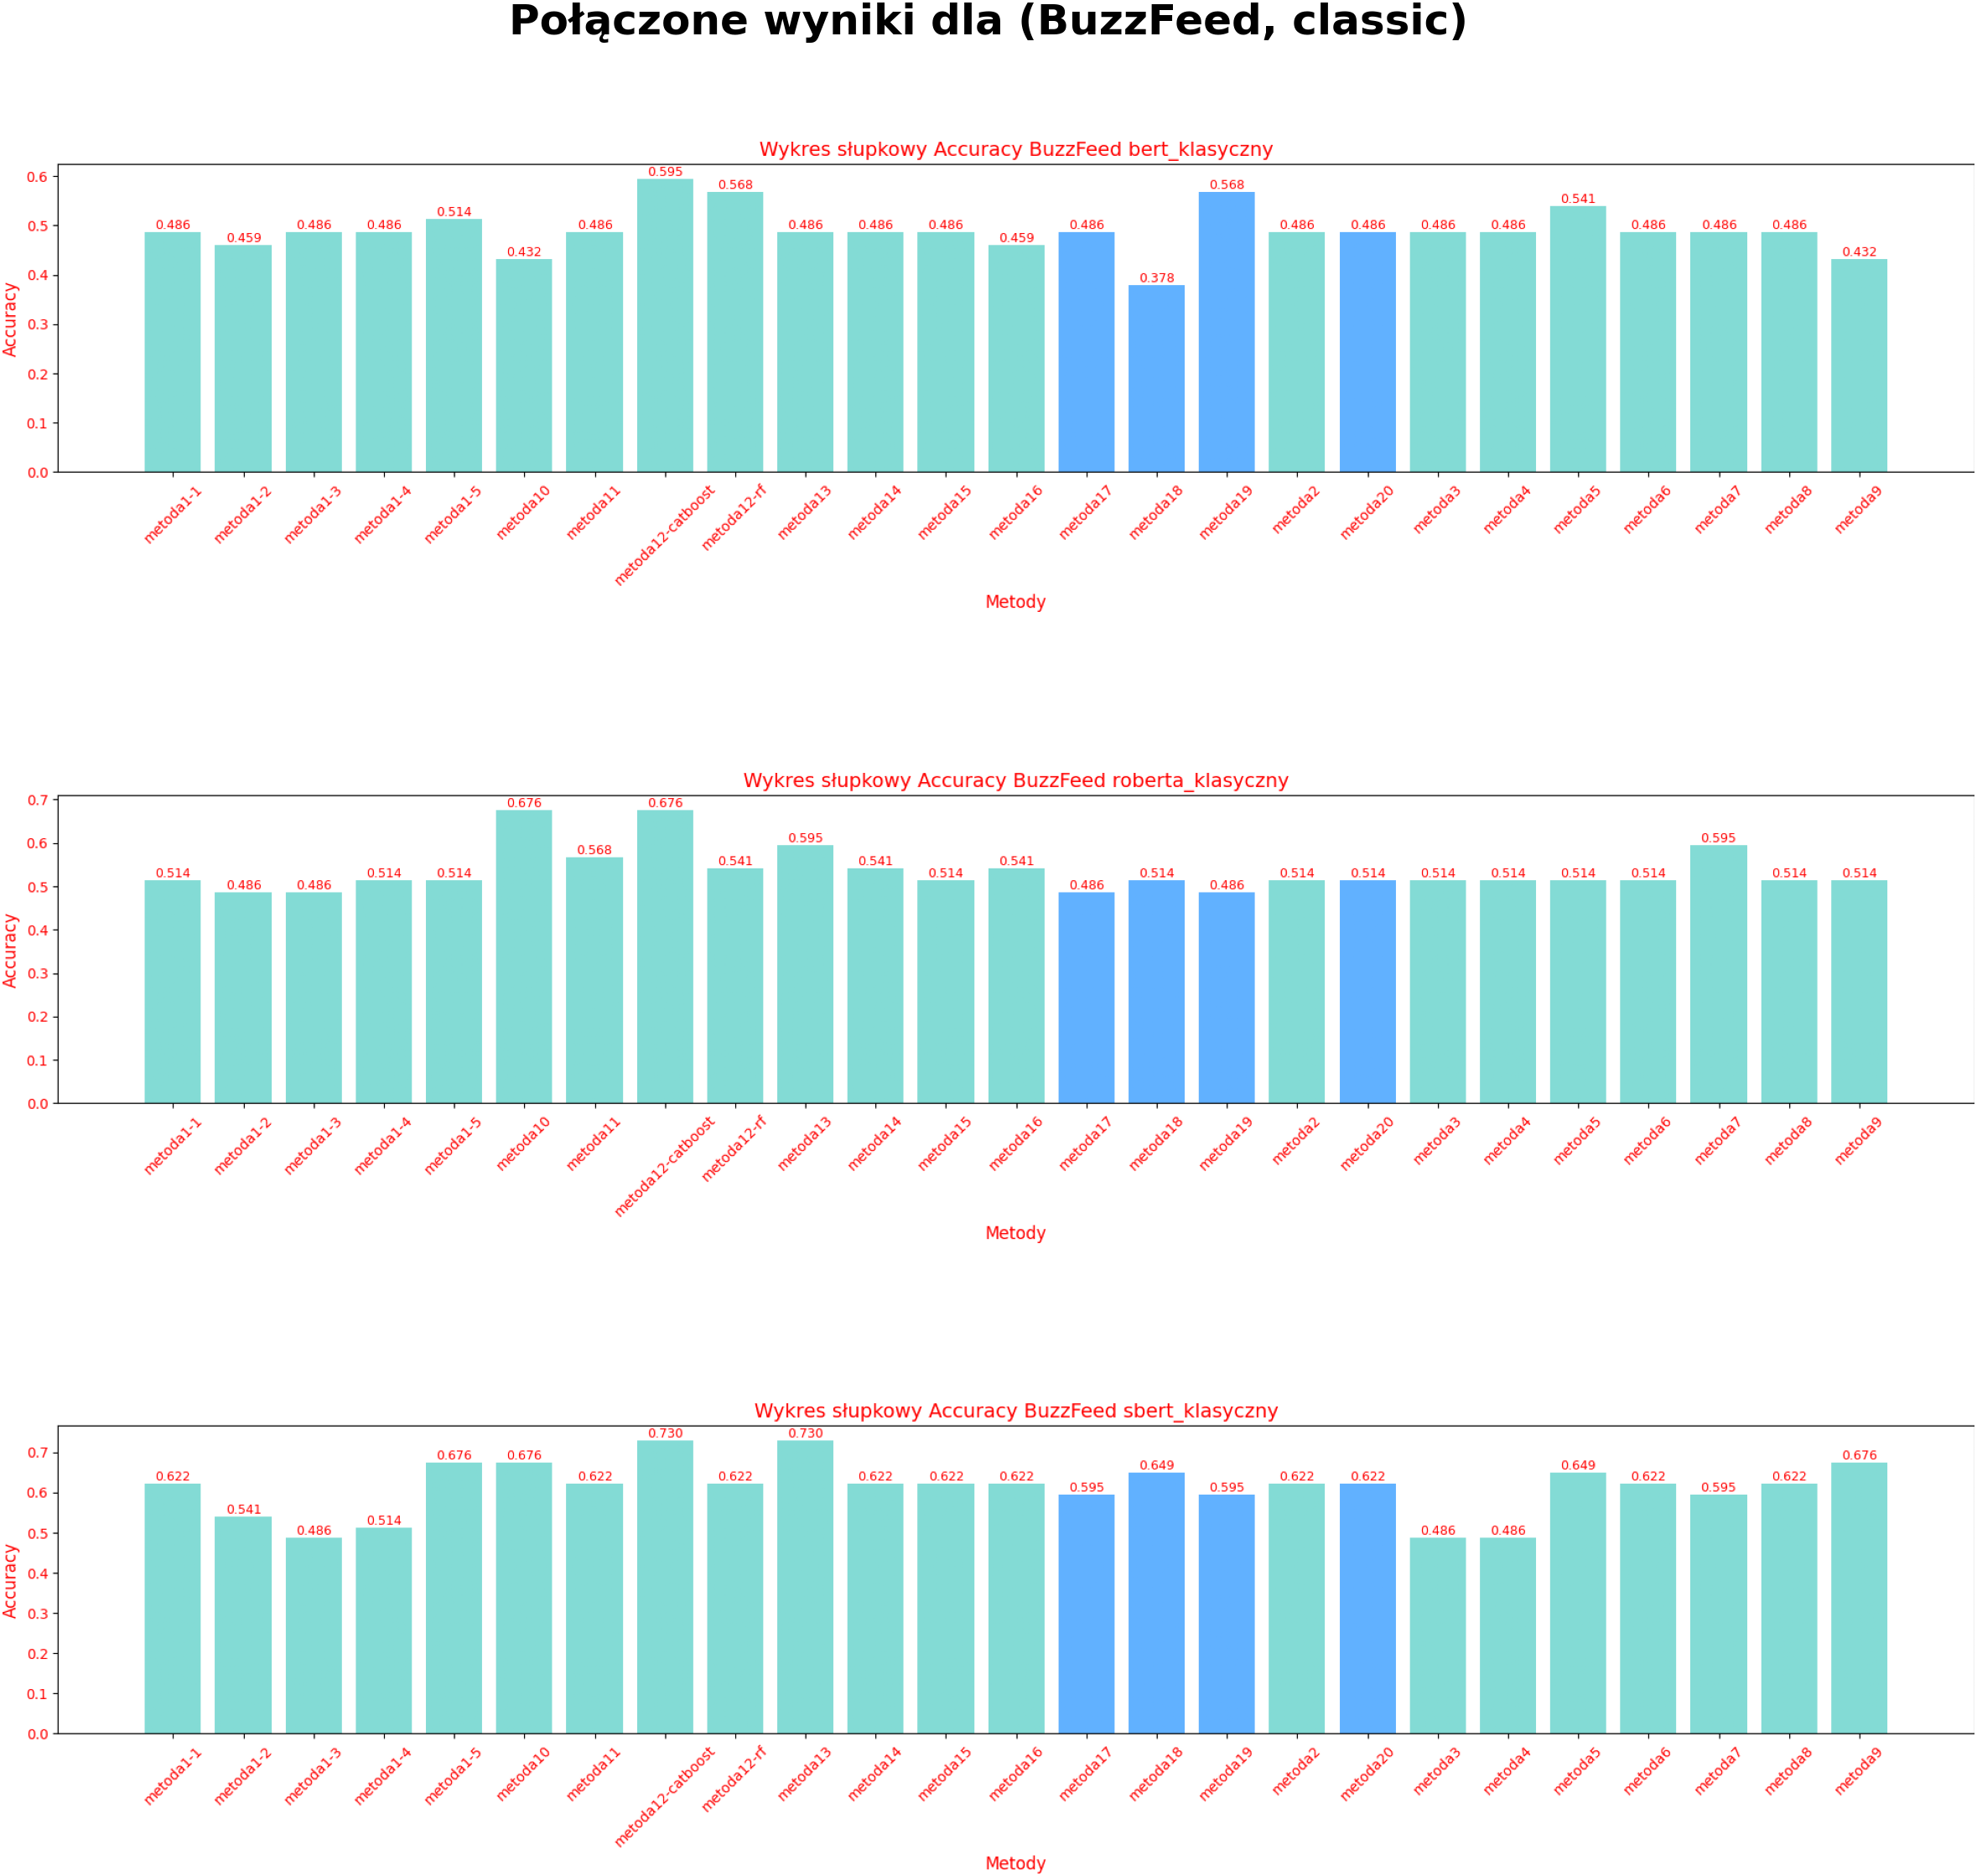
\includegraphics[width=0.99\textwidth]{img/stats/BuzzFeed_classic/BuzzFeed_classic_Combined_Accuracy_bar_chart.png}
	\caption{Histogram rozkładu \textbf{Dokładności (Accuracy)}.}
	\label{fig:buzzfeed_classic_accuracy}
\end{figure}

\subsubsection{F1-Score}
Wykresy F1-Score (\ref{fig:buzzfeed_classic_f1}) wskazują, że dla BERT \texttt{Metoda19}, \texttt{Metoda17}, \texttt{Metoda12-catboost} osiągnęły najwyższe wartości, a \texttt{Metoda1-2}, \texttt{Metoda1-5} najniższe. Dla RoBERTa \texttt{Metoda1-2}, \texttt{Metoda10}, \texttt{Metoda17} były najlepsze, a \texttt{Metoda1-1}, \texttt{Metoda1-4} najgorsze. Dla SBERT \texttt{Metoda13}, \texttt{Metoda12-catboost}, \texttt{Metoda18}, \texttt{Metoda19} osiągnęły wysokie wyniki, a \texttt{Metoda1-2} najniższe. \texttt{Metoda17} osiąga wysoki F1 dla RoBERTa dzięki VotingClassifier, \texttt{Metoda18} dobrze radzi sobie dla SBERT z powodu stacking z CatBoost, \texttt{Metoda19} jest skuteczna dla BERT/SBERT dzięki modelom ensemble, a \texttt{Metoda20} średnia z powodu braku optymalizacji.

\begin{figure}[H]
	\centering
	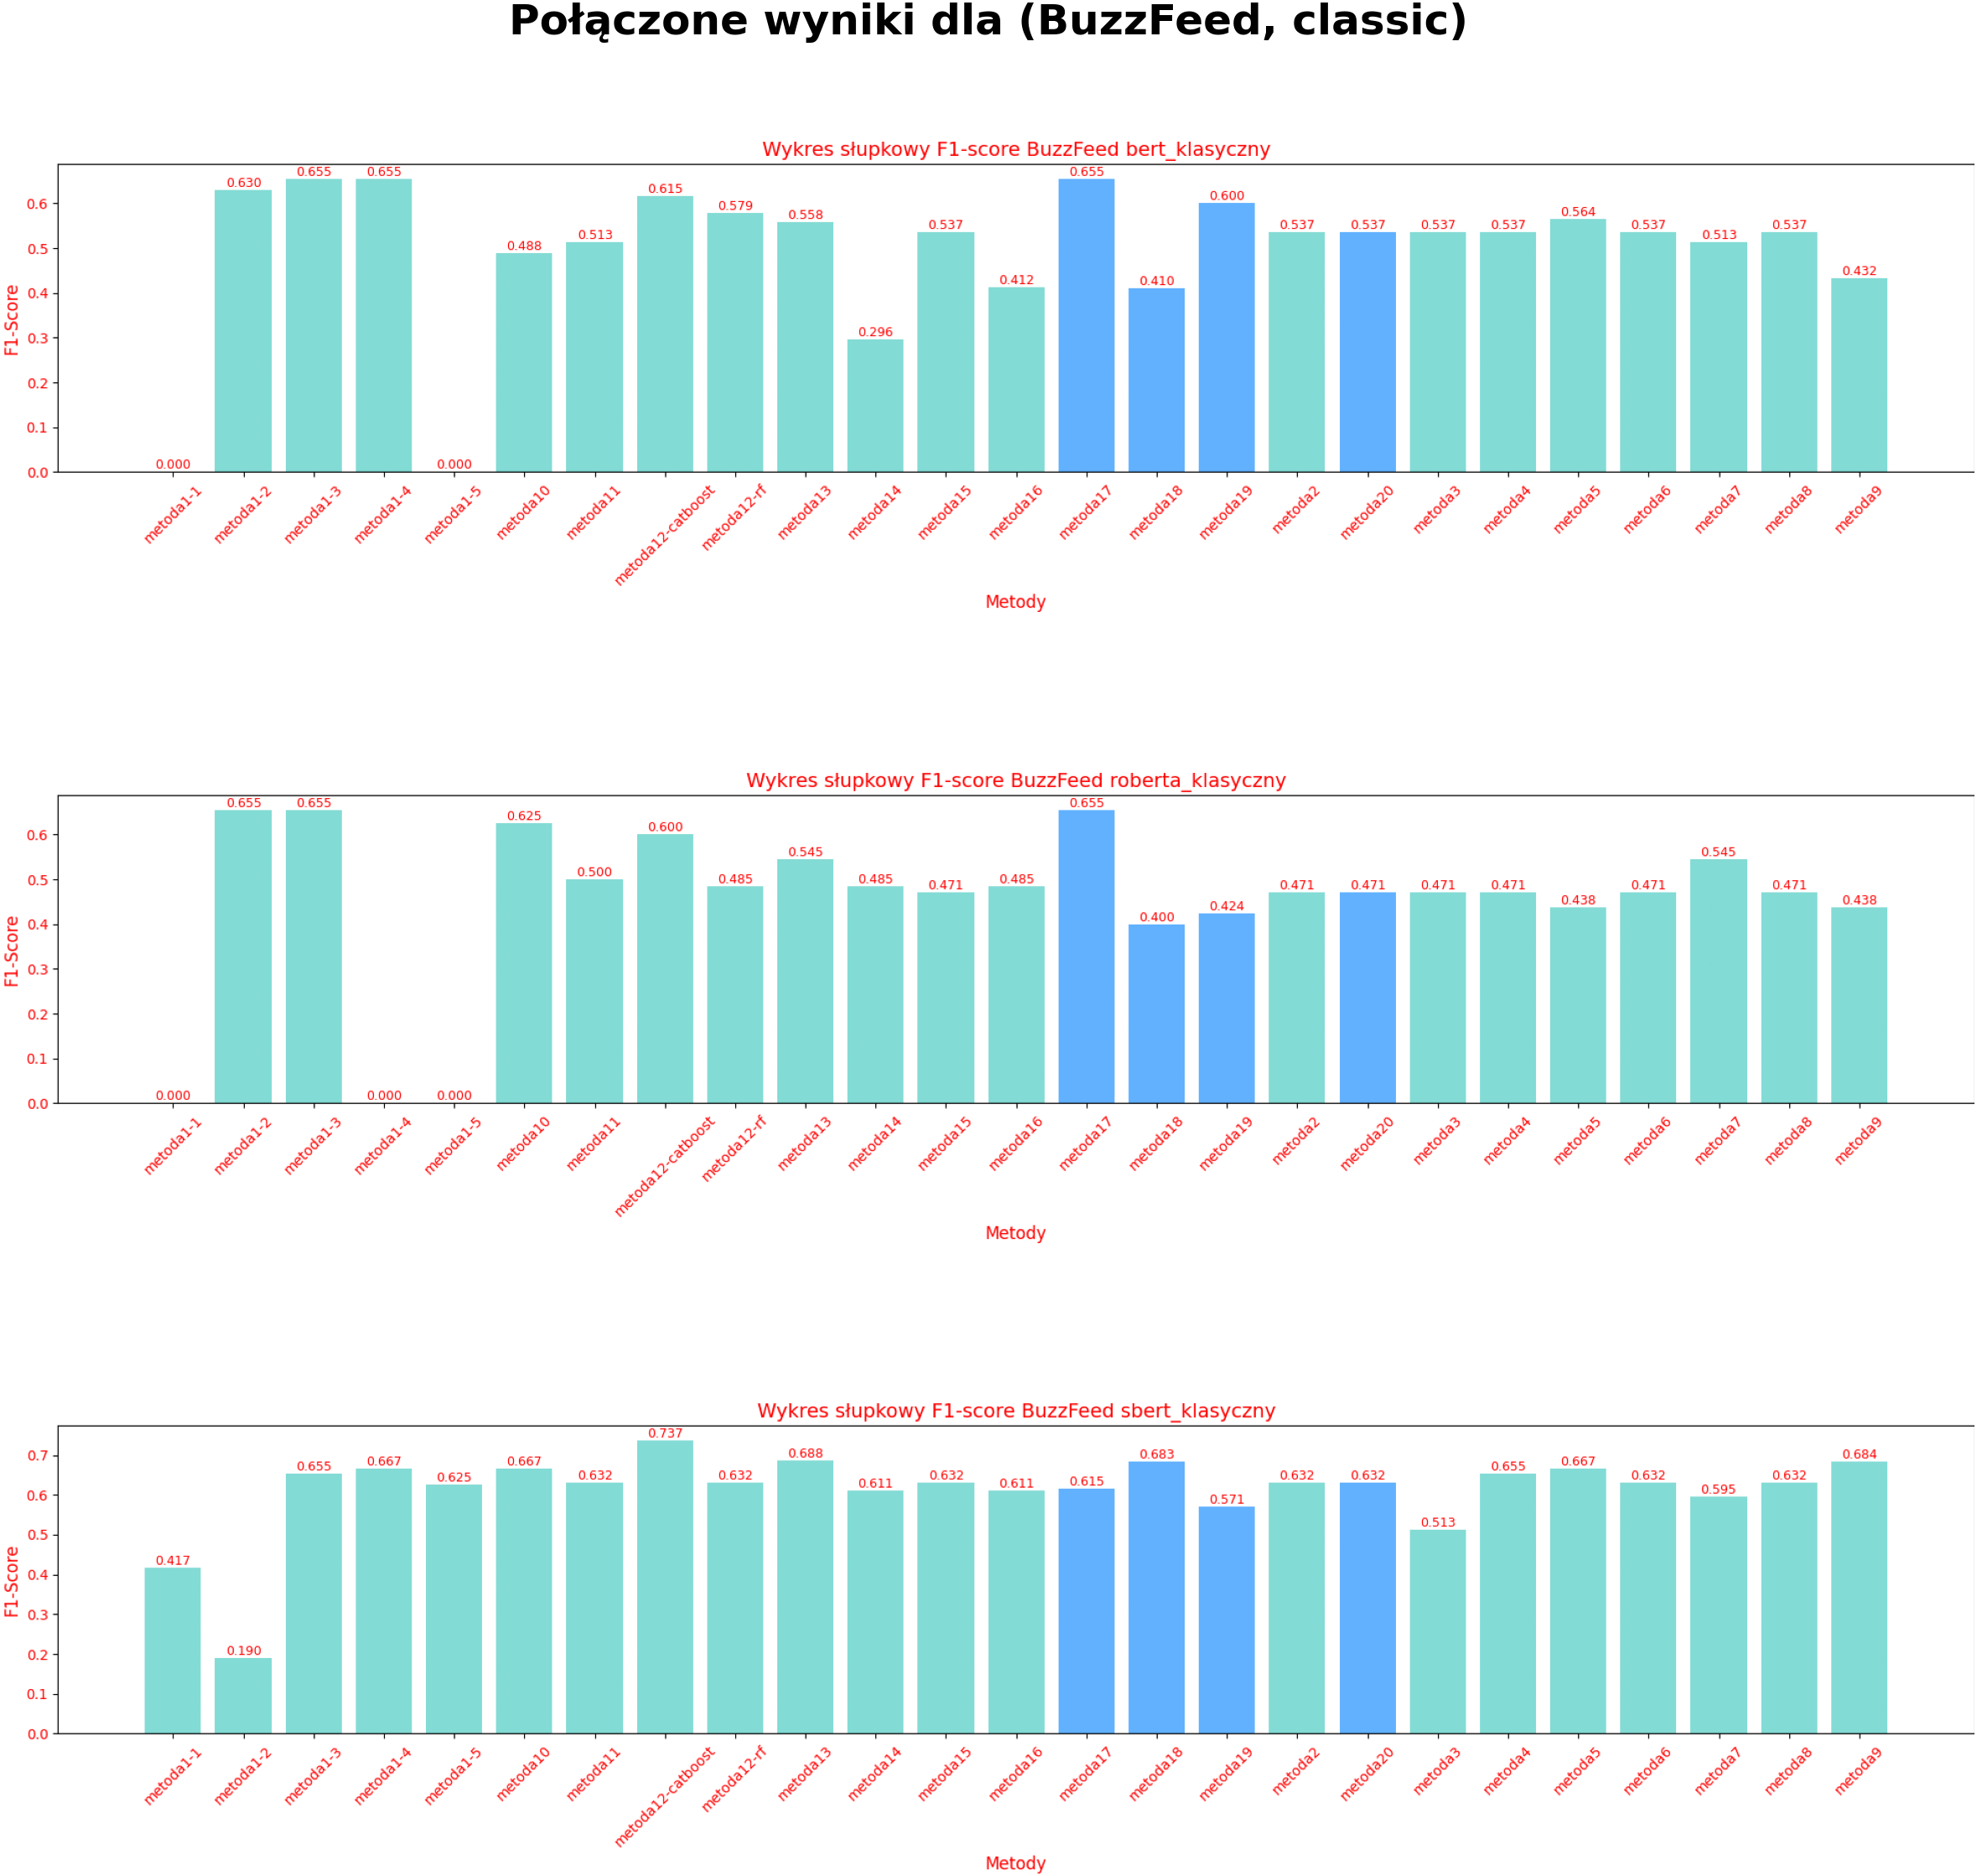
\includegraphics[width=0.99\textwidth]{img/stats/BuzzFeed_classic/BuzzFeed_classic_Combined_F1-Score_bar.png}
	\caption{Histogram rozkładu \textbf{Wyniku F1 (F1-Score)}.}
	\label{fig:buzzfeed_classic_f1}
\end{figure}

\subsubsection{ROC-AUC}
Wykresy ROC-AUC (\ref{fig:buzzfeed_classic_roc}) pokazują, że dla BERT \texttt{Metoda19} osiągnęła najwyższe wartości, a \texttt{Metoda17}, \texttt{Metoda1-4} najniższe. Dla RoBERTa \texttt{Metoda1-2}, \texttt{Metoda1-3}, \texttt{Metoda17} były najlepsze, a \texttt{Metoda14}, \texttt{Metoda19} najgorsze. Dla SBERT \texttt{Metoda1-4} osiągnęła wysoki wynik, a \texttt{Metoda4} najniższy. \texttt{Metoda17} jest skuteczna dla RoBERTa dzięki VotingClassifier, \texttt{Metoda18} słaba dla BERT z powodu prostej konfiguracji, \texttt{Metoda19} dominuje dla BERT dzięki stacking, a \texttt{Metoda20} średnia z powodu braku balansowania.

\begin{figure}[H]
	\centering
	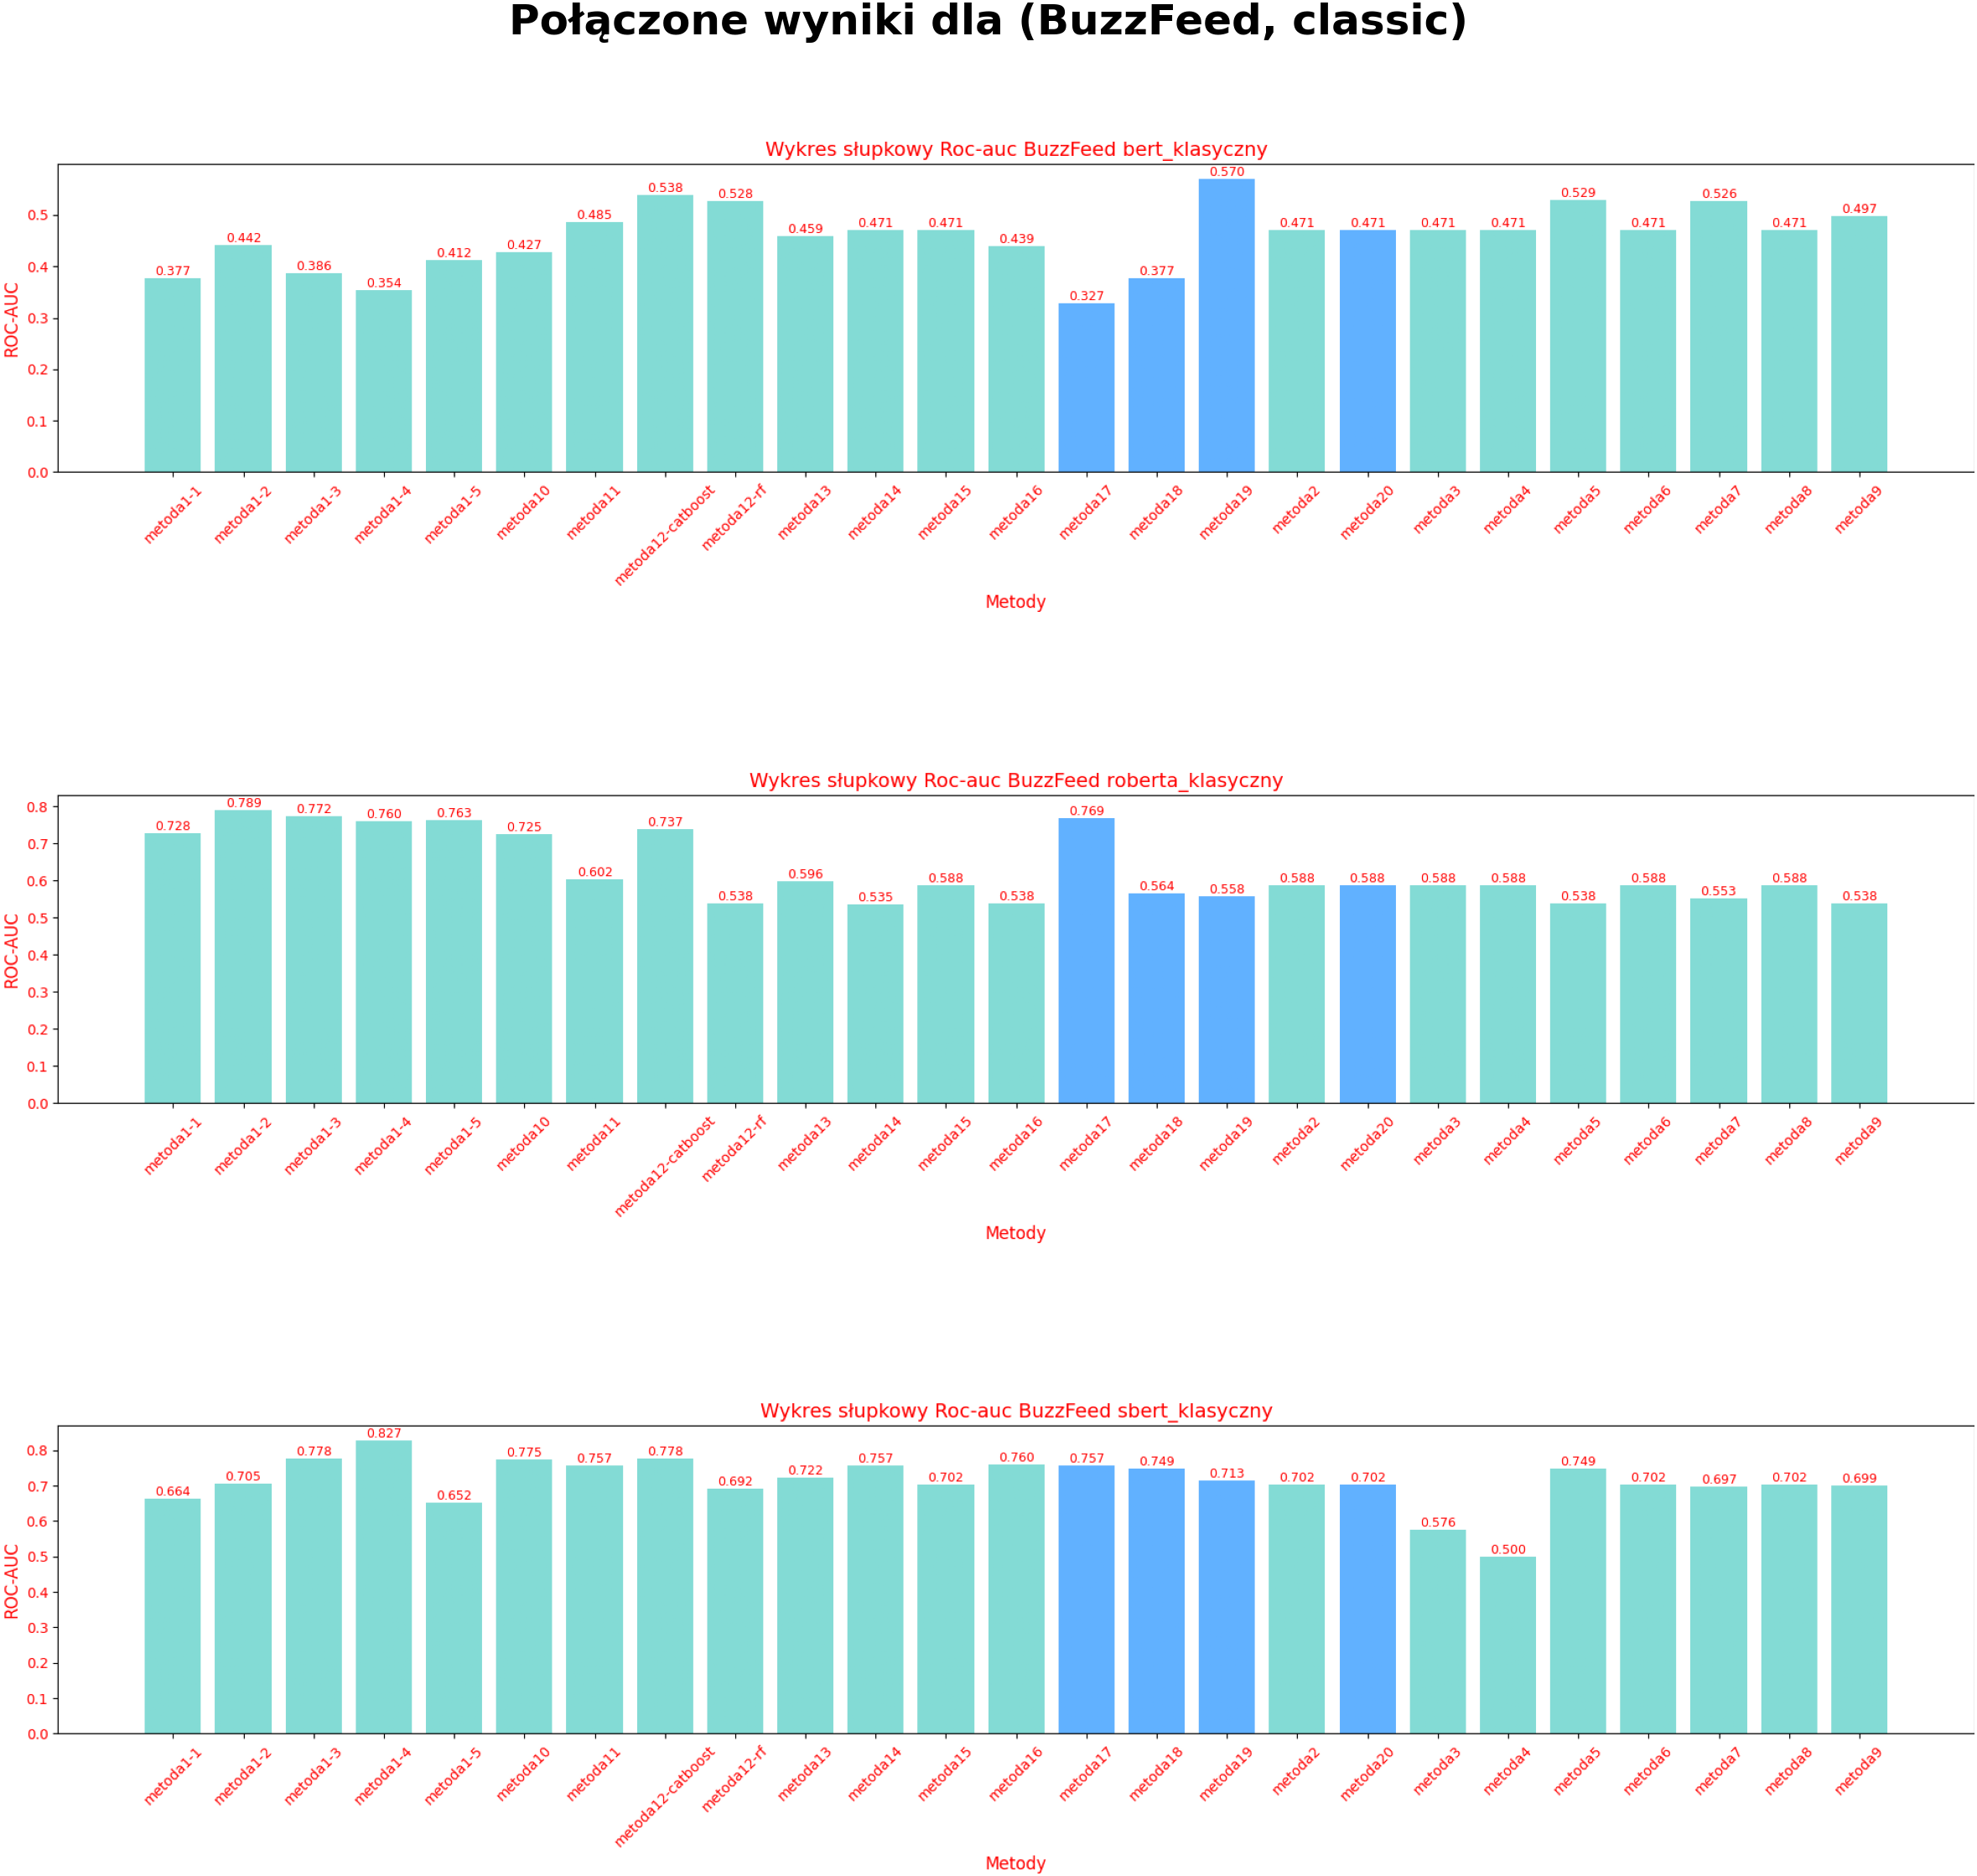
\includegraphics[width=0.99\textwidth]{img/stats/BuzzFeed_classic/BuzzFeed_classic_Combined_ROC-AUC_bar.png}
	\caption{Histogram rozkładu \textbf{Pola pod krzywą ROC-AUC (ROC-AUC)}.}
	\label{fig:buzzfeed_classic_roc}
\end{figure}

\subsection{Wyniki w trybie few-shot}

\subsubsection{Accuracy}
Wykresy Accuracy (\ref{fig:buzzfeed_few_shot_accuracy}) wskazują, że dla BERT \texttt{Metoda13}, \texttt{Metoda14}, \texttt{Metoda19} osiągnęły najlepsze wyniki, a \texttt{Metoda12-rf} najgorsze. Dla RoBERTa \texttt{Metoda18} była najlepsza, a \texttt{Metoda15}, \texttt{Metoda20} najsłabsze. Dla SBERT \texttt{Metoda19}, \texttt{Metoda5}, \texttt{Metoda13} osiągnęły ~0.7, a \texttt{Metoda12-rf} ~0.5. \texttt{Metoda17} słaba dla BERT z powodu niedopasowania VotingClassifier, \texttt{Metoda18} skuteczna dla RoBERTa dzięki stacking z CatBoost, \texttt{Metoda19} wysoka dla BERT/SBERT dzięki ensemble, \texttt{Metoda20} słaba dla RoBERTa z powodu braku optymalizacji.

\begin{figure}[H]
	\centering
	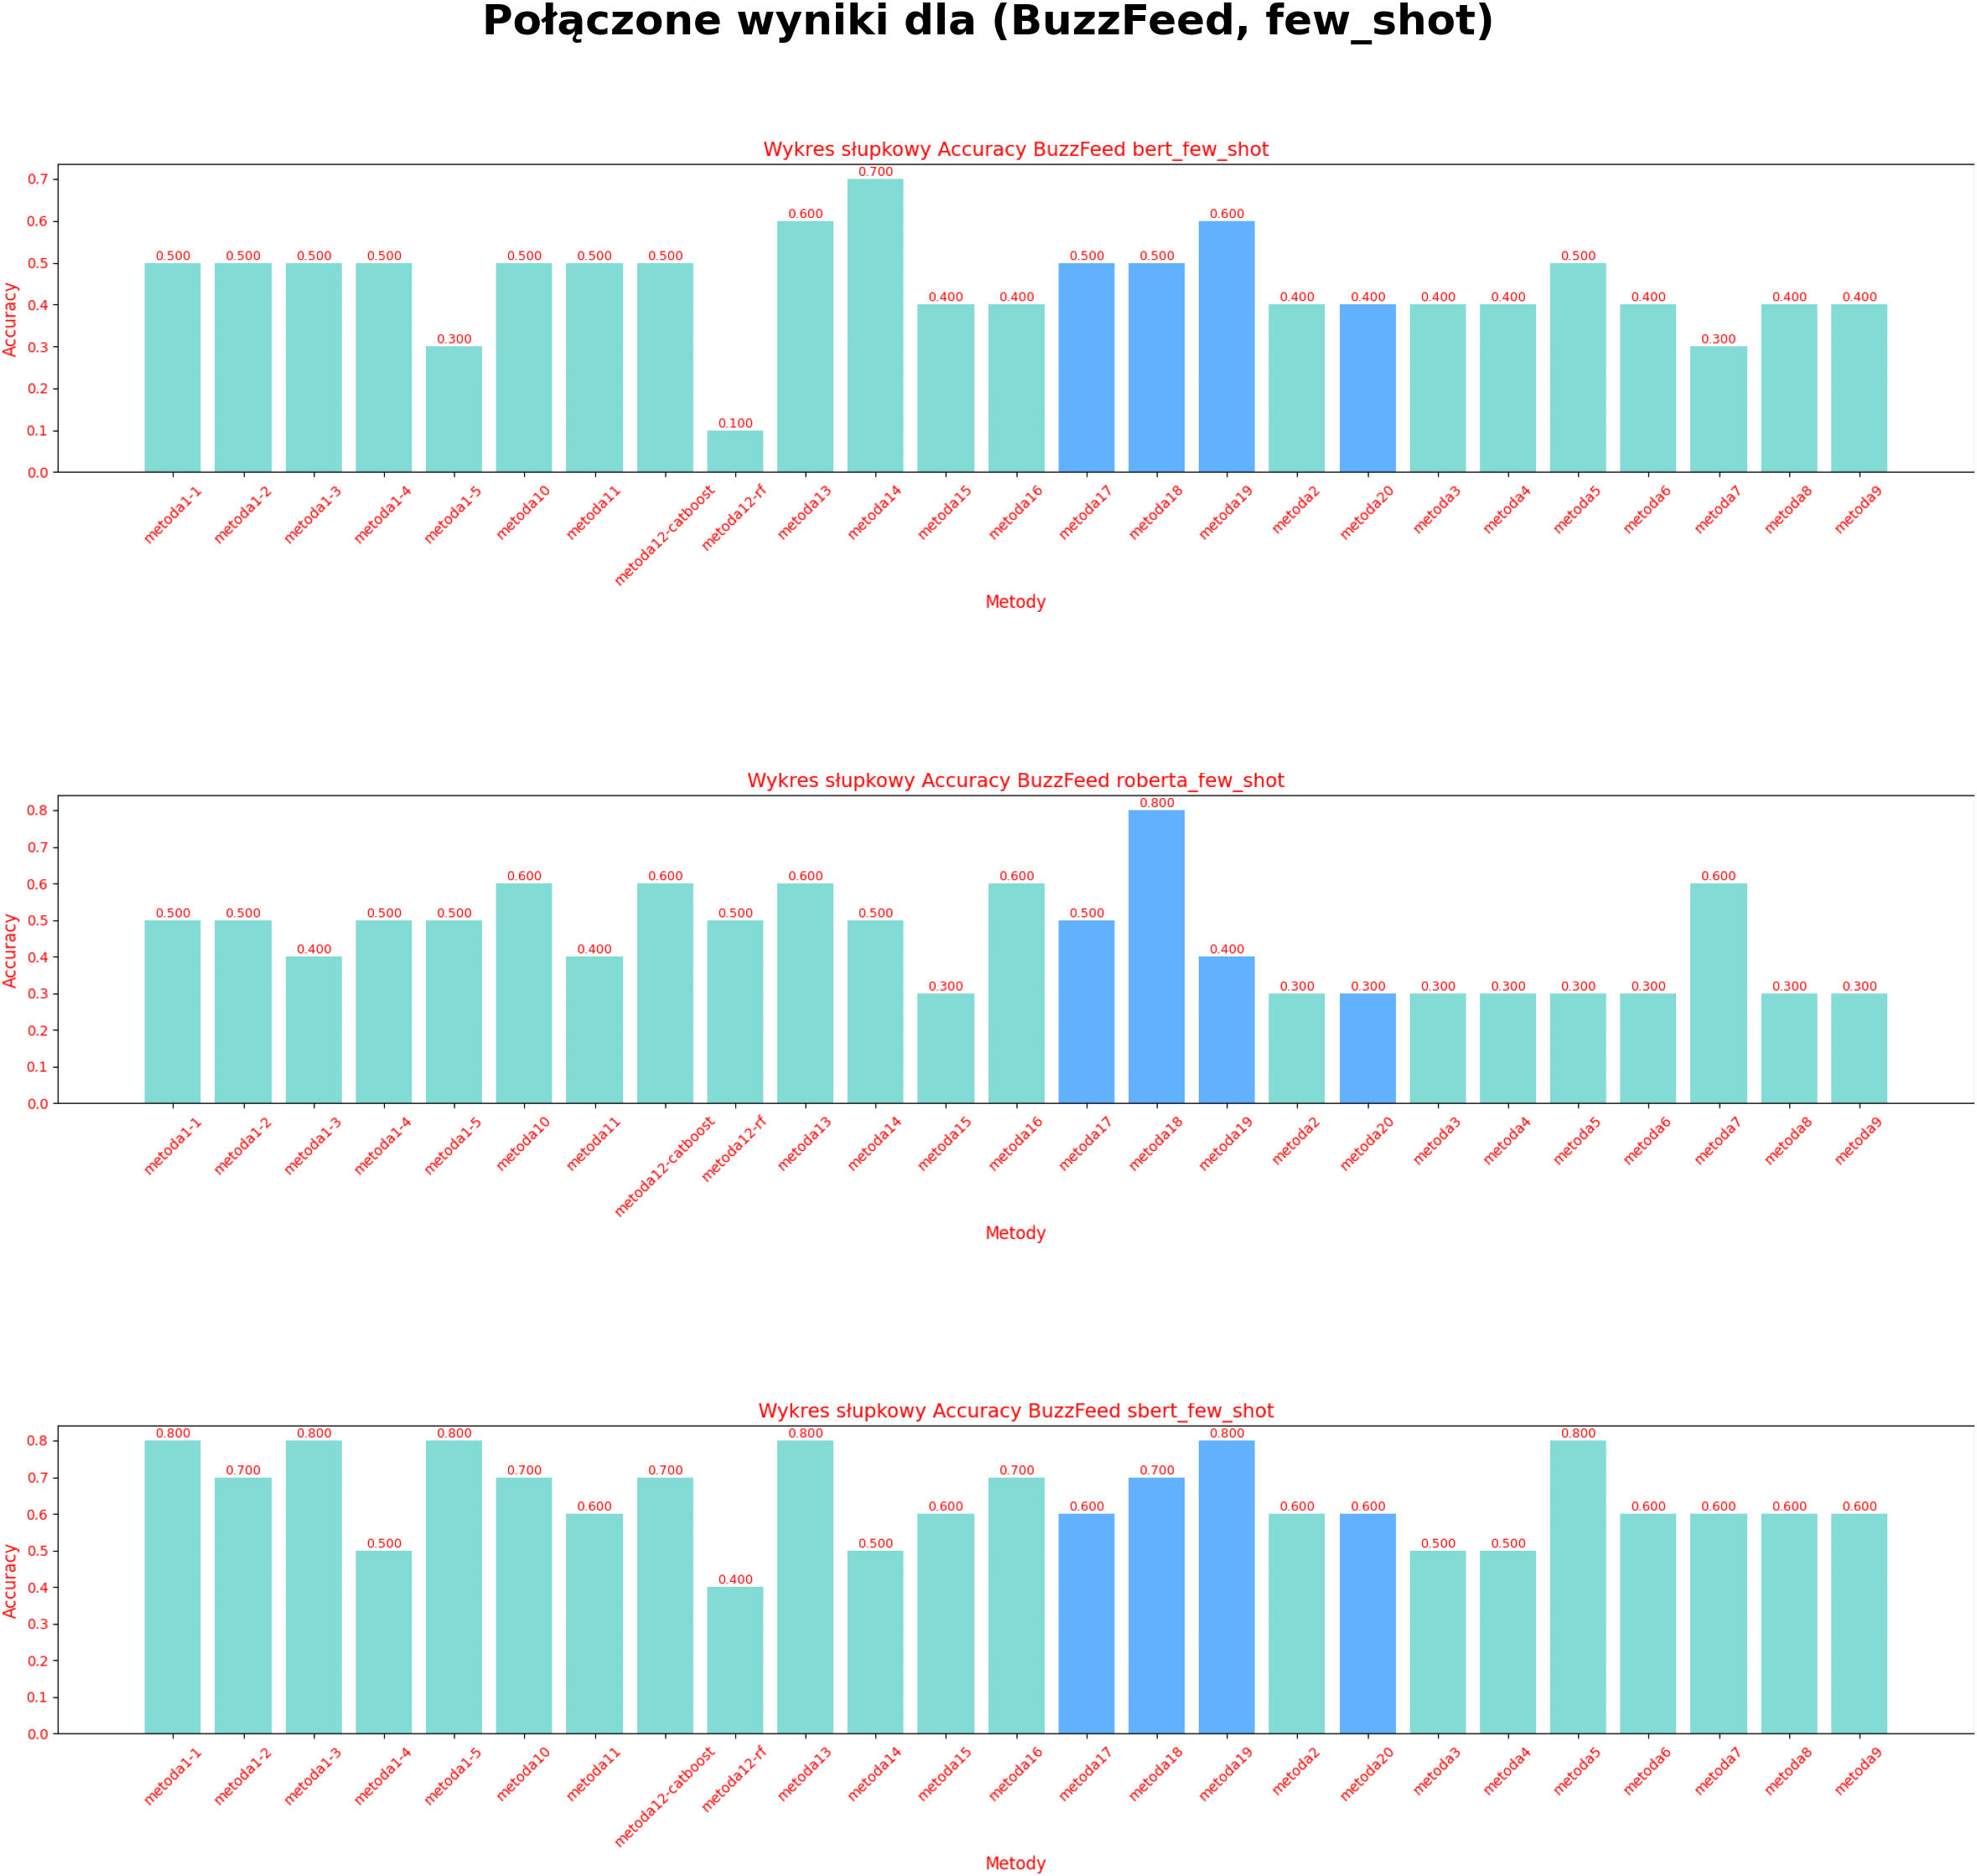
\includegraphics[width=0.99\textwidth]{img/stats/BuzzFeed_few_shot/BuzzFeed_few_shot_Combined_Accuracy_bar_chart.png}
	\caption{Histogram rozkładu \textbf{Dokładności (Accuracy)}.}
	\label{fig:buzzfeed_few_shot_accuracy}
\end{figure}

\subsubsection{F1-Score}
Wykresy F1-Score (\ref{fig:buzzfeed_few_shot_f1}) pokazują, że dla BERT \texttt{Metoda19}, \texttt{Metoda14} osiągnęły najwyższe wartości, a \texttt{Metoda17} najniższe. Dla RoBERTa \texttt{Metoda18} była najlepsza, a \texttt{Metoda20}, \texttt{Metoda17} najgorsze. Dla SBERT \texttt{Metoda13}, \texttt{Metoda19} osiągnęły wysokie wyniki, a \texttt{Metoda3} najniższe. \texttt{Metoda17} słaba dla BERT/RoBERTa z powodu VotingClassifier, \texttt{Metoda18} skuteczna dla RoBERTa dzięki stacking, \texttt{Metoda19} wysoka dla BERT/SBERT dzięki ensemble, \texttt{Metoda20} słaba dla RoBERTa z braku balansowania.

\begin{figure}[H]
	\centering
	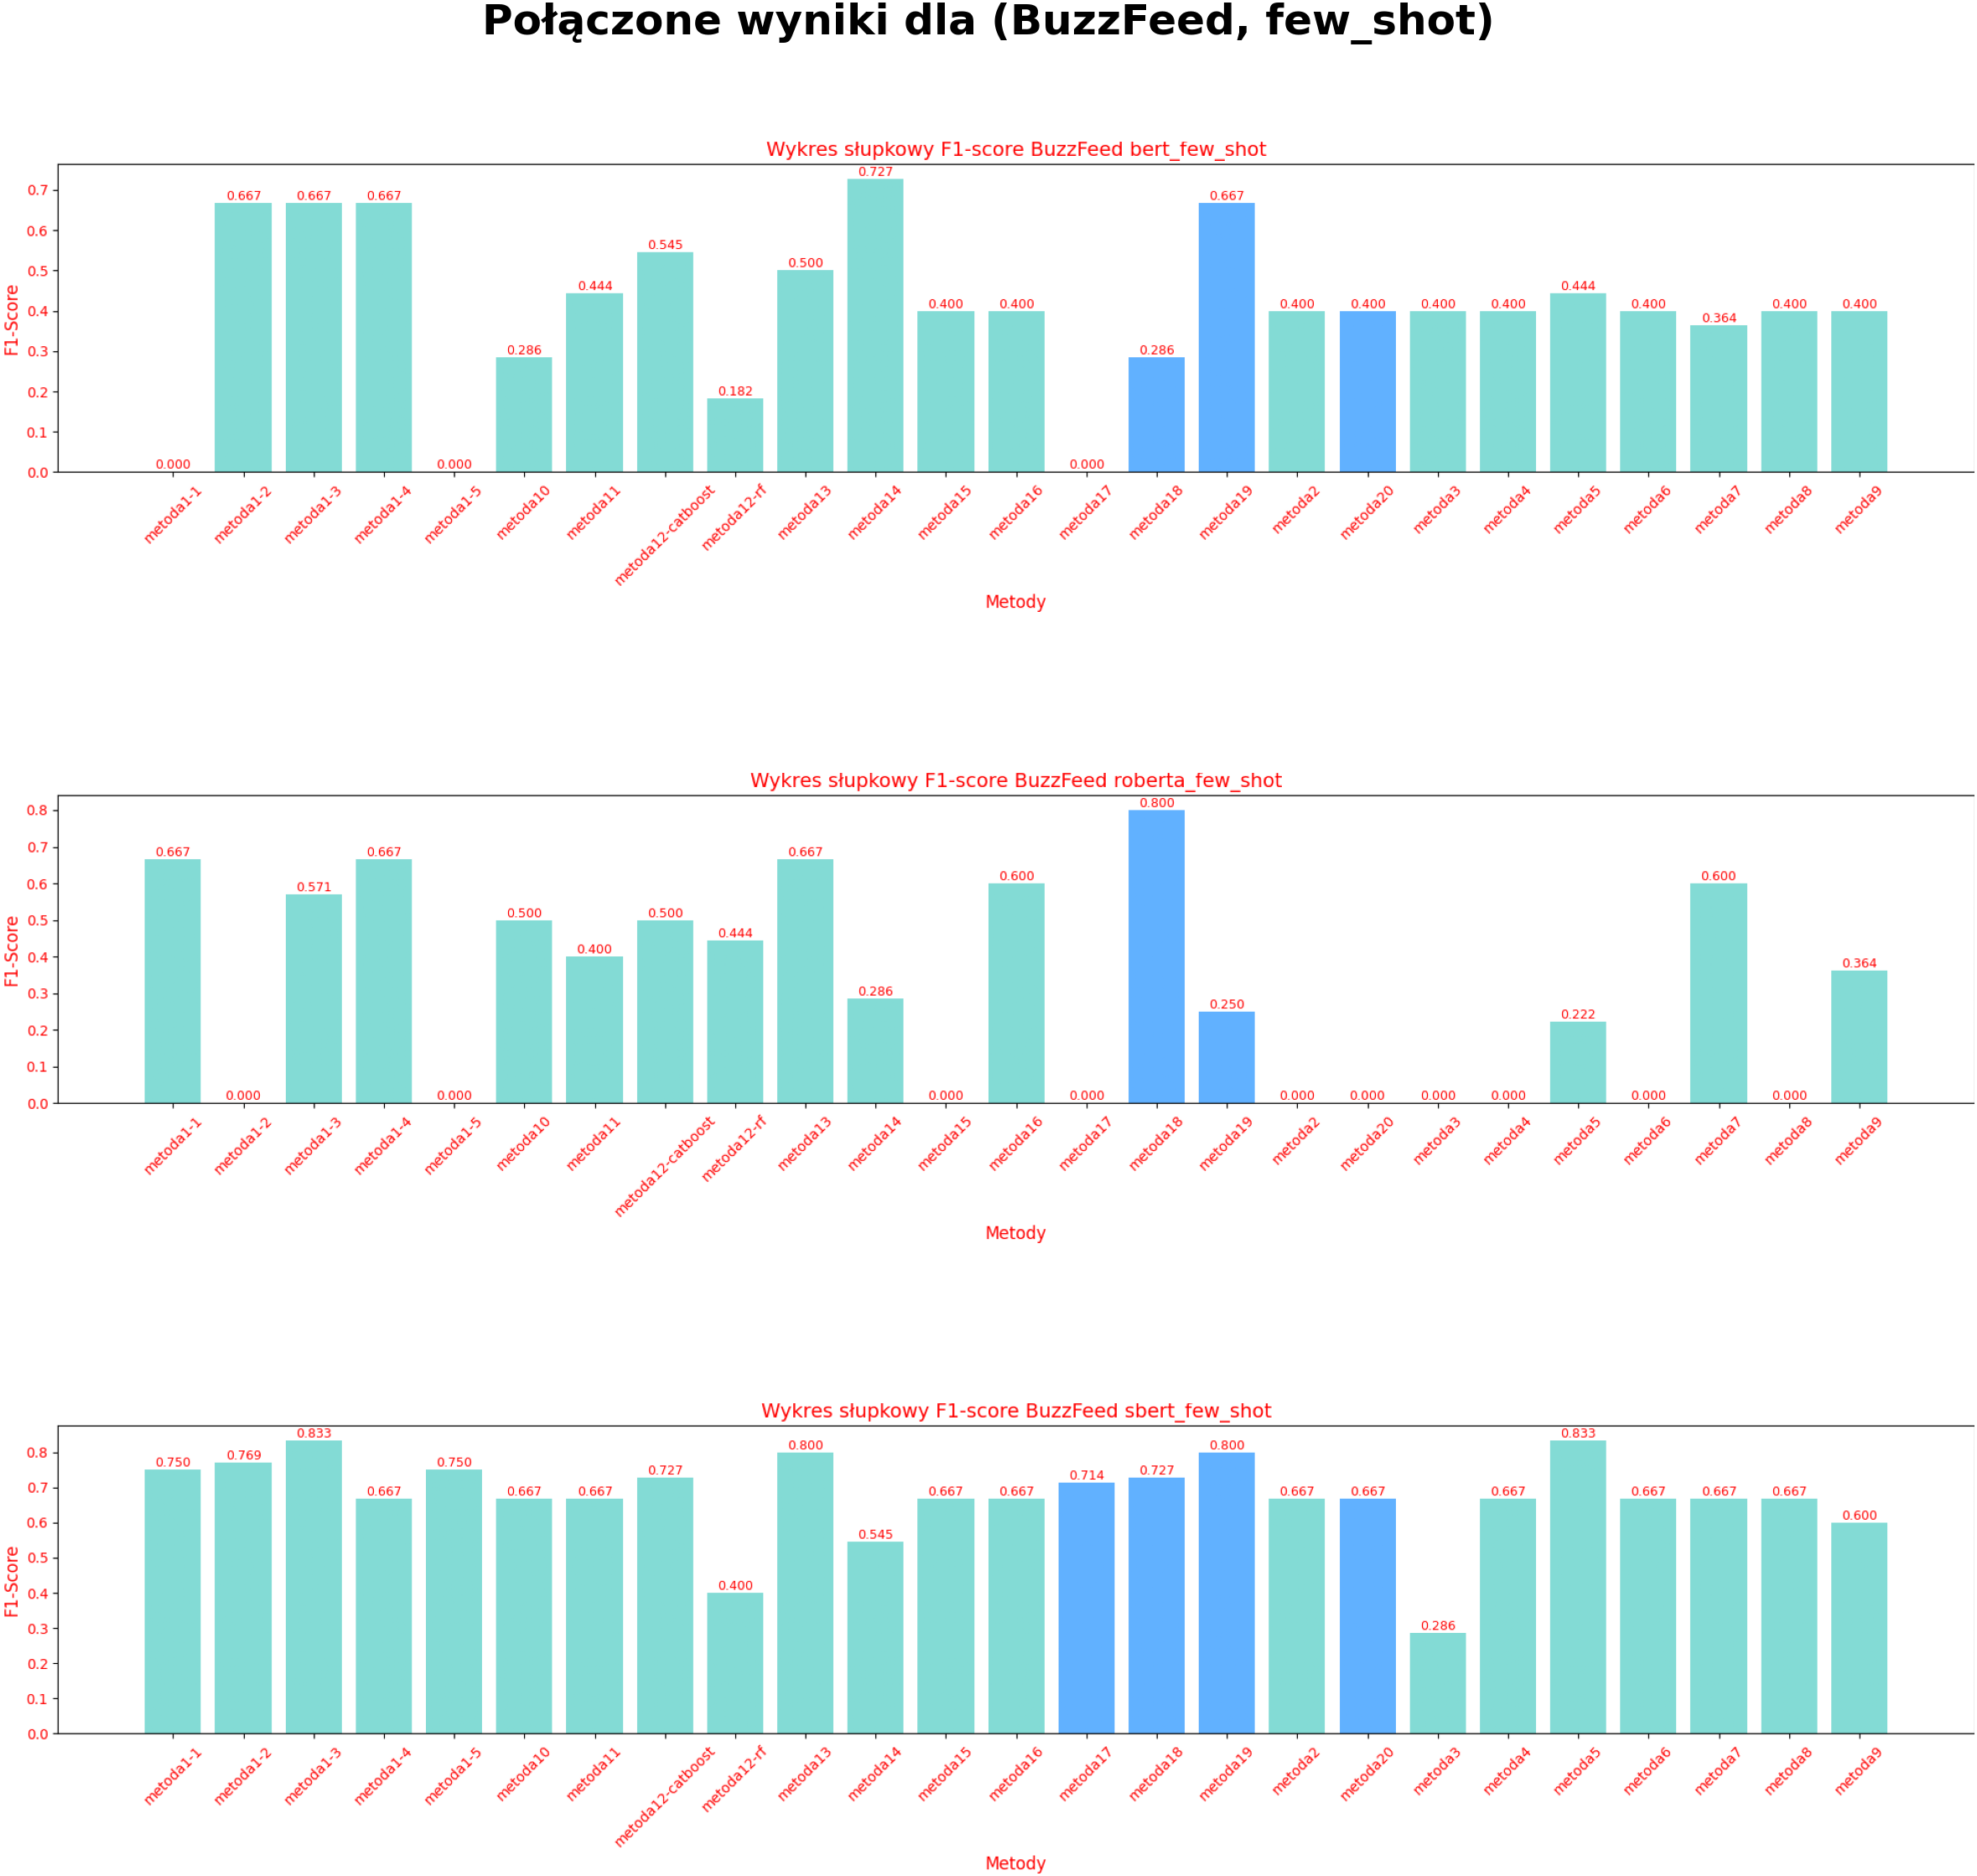
\includegraphics[width=0.99\textwidth]{img/stats/BuzzFeed_few_shot/BuzzFeed_few_shot_Combined_F1-Score_bar.png}
	\caption{Histogram rozkładu \textbf{Wyniku F1 (F1-Score)}.}
	\label{fig:buzzfeed_few_shot_f1}
\end{figure}

\subsubsection{ROC-AUC}
Wykresy ROC-AUC (\ref{fig:buzzfeed_few_shot_roc}) wskazują, że dla BERT \texttt{Metoda14} osiągnęła najwyższe wartości, a \texttt{Metoda16}, \texttt{Metoda20} najniższe. Dla RoBERTa \texttt{Metoda17}, \texttt{Metoda18} były najlepsze, a \texttt{Metoda19} najgorsza. Dla SBERT \texttt{Metoda19}, \texttt{Metoda5} osiągnęły wysokie wyniki, a \texttt{Metoda14} najniższe. \texttt{Metoda17} skuteczna dla RoBERTa dzięki VotingClassifier, \texttt{Metoda18} wysoka dla RoBERTa dzięki stacking, \texttt{Metoda19} słaba dla RoBERTa z braku optymalizacji, \texttt{Metoda20} słaba dla BERT z powodu prostej konfiguracji.

\begin{figure}[H]
	\centering
	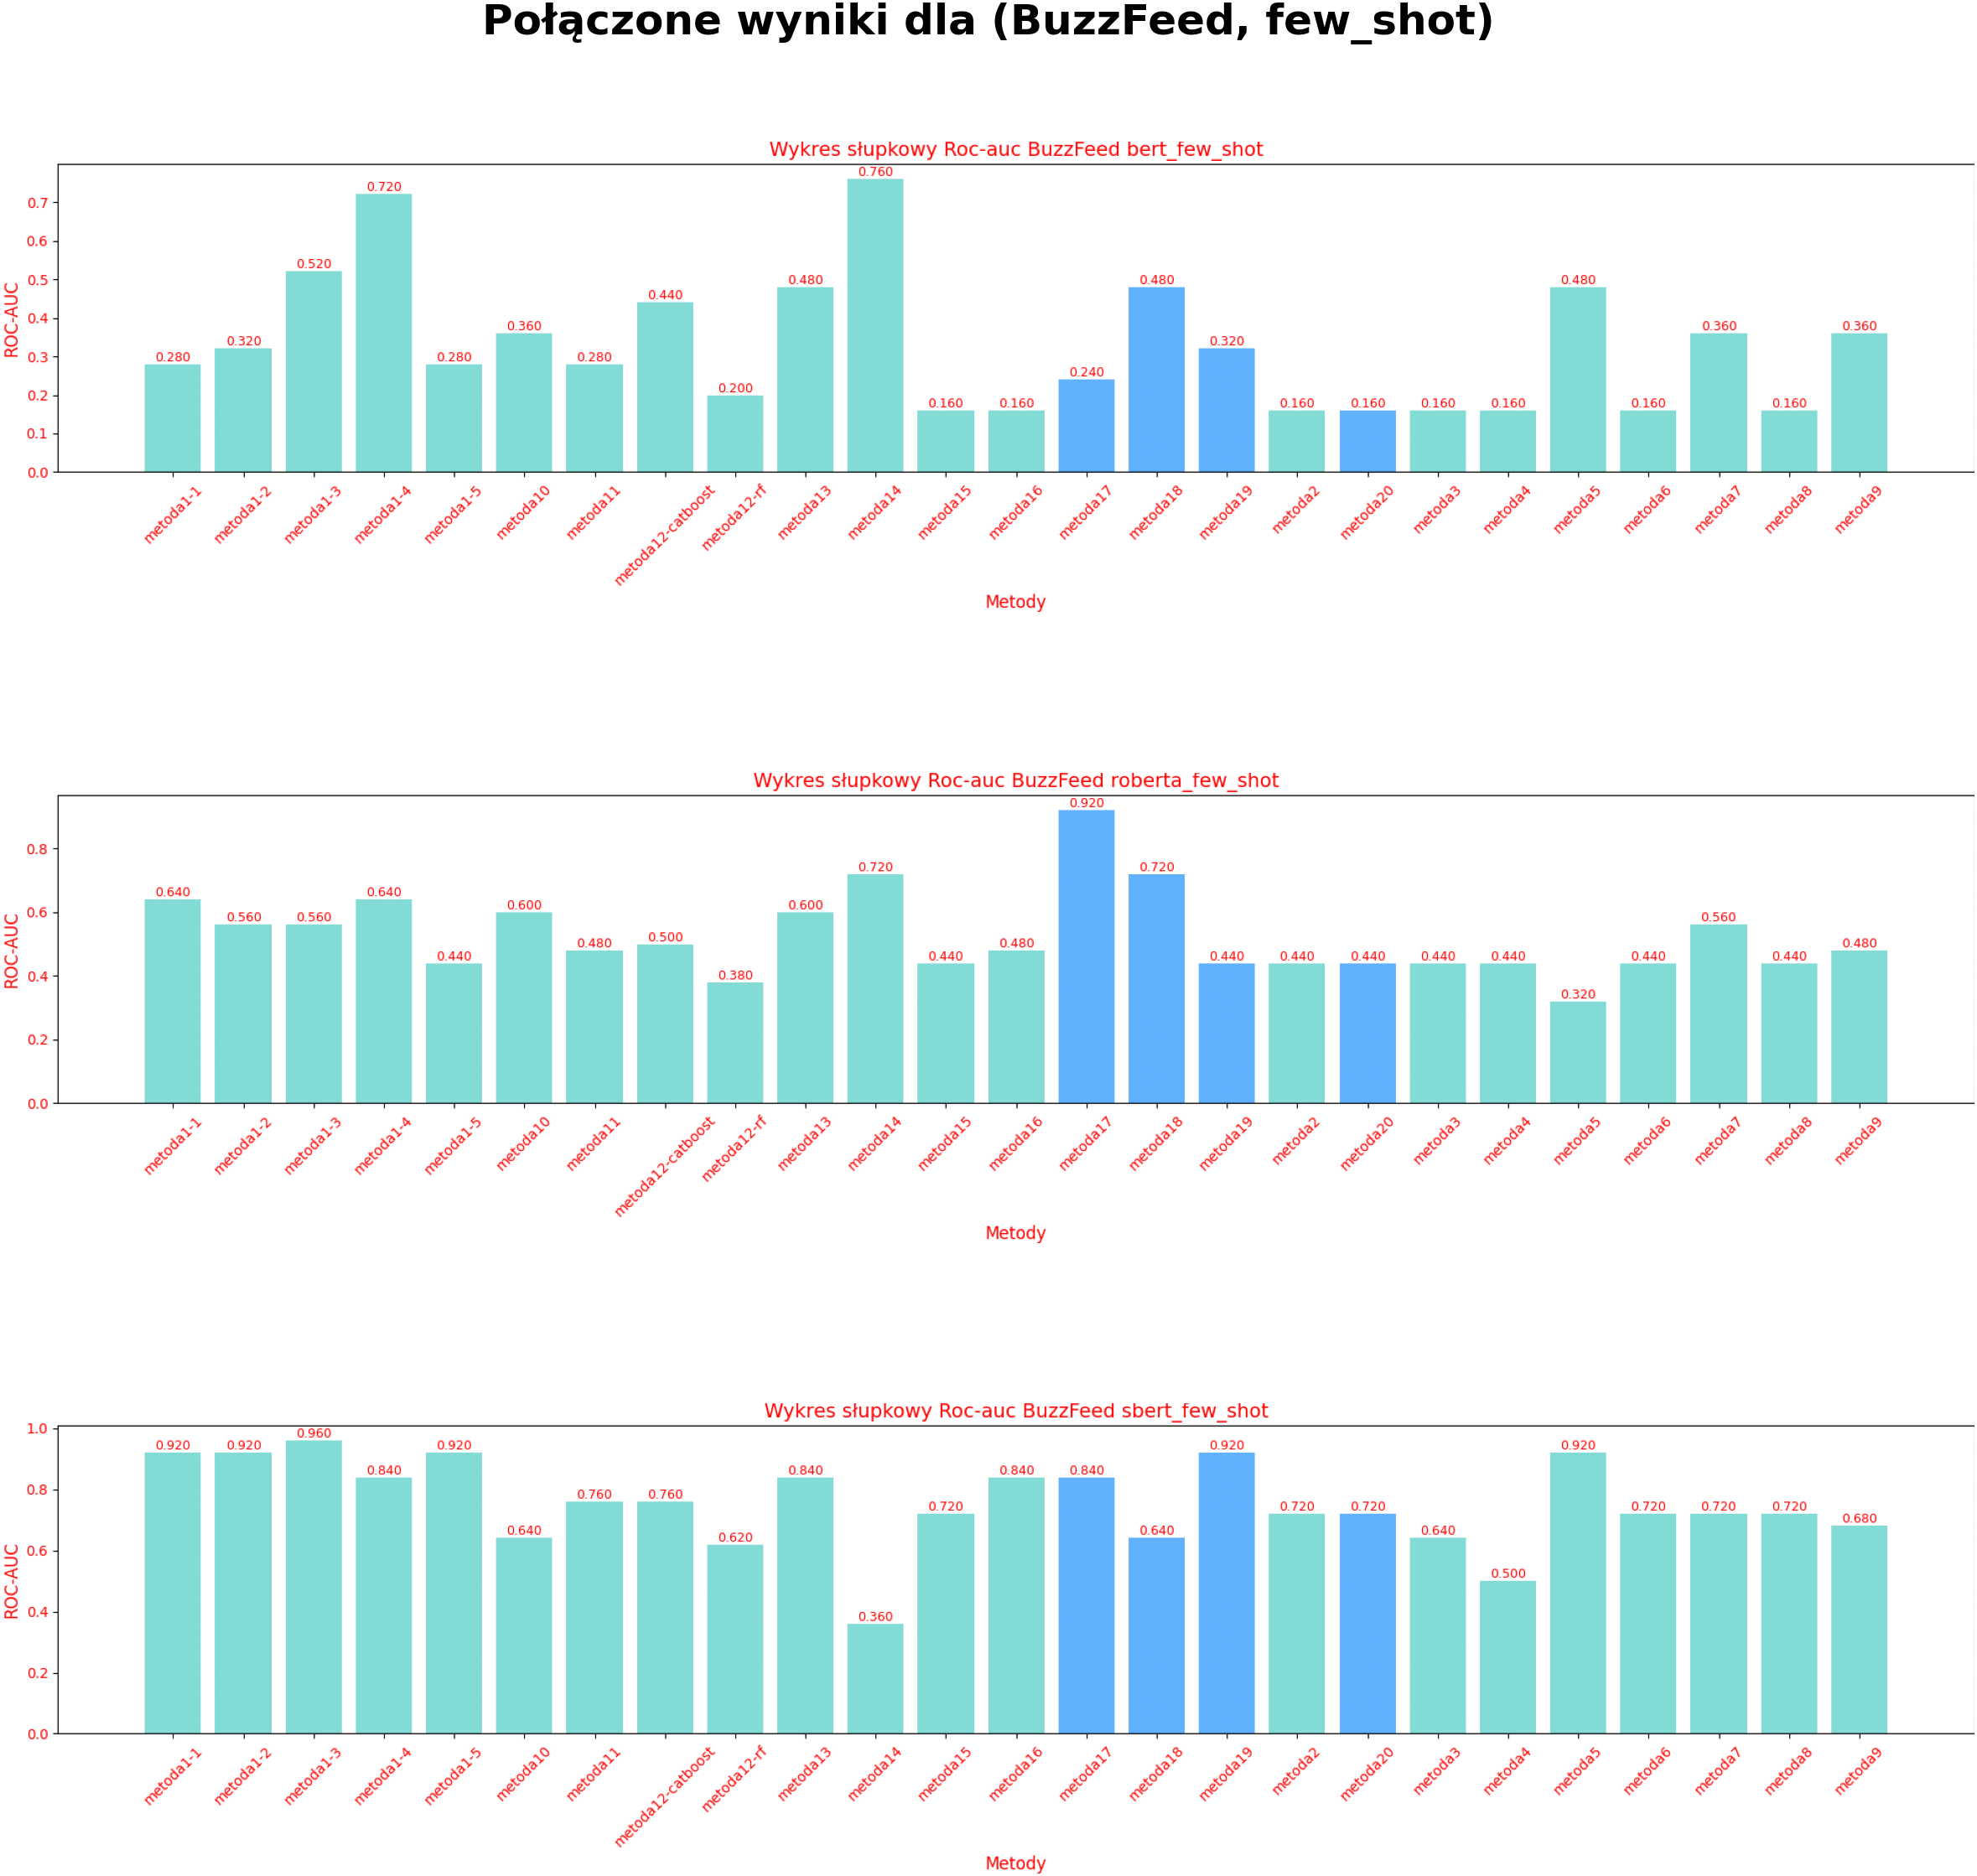
\includegraphics[width=0.99\textwidth]{img/stats/BuzzFeed_few_shot/BuzzFeed_few_shot_Combined_ROC-AUC_bar.png}
	\caption{Histogram rozkładu \textbf{Pola pod krzywą ROC-AUC (ROC-AUC)}.}
	\label{fig:buzzfeed_few_shot_roc}
\end{figure}

\subsection{Wyniki w trybie one-shot}

\subsubsection{Accuracy}
Wykresy Accuracy (\ref{fig:buzzfeed_one_shot_accuracy}) pokazują, że dla BERT \texttt{Metoda12-catboost}, \texttt{Metoda20} osiągnęły ~100\%, a pozostałe ~50\%. Dla RoBERTa \texttt{Metoda12-catboost}, \texttt{Metoda19} miały ~100\%, a reszta ~50\%. Dla SBERT \texttt{Metoda}1-1, \texttt{Metoda20} osiągnęły ~100\%, a inne ~50\%. \texttt{Metoda17}, \texttt{Metoda18}, \texttt{Metoda19} słabe dla BERT z powodu niedostatecznej adaptacji, \texttt{Metoda20} skuteczna dzięki zoptymalizowanemu LightGBM.

\begin{figure}[H]
	\centering
	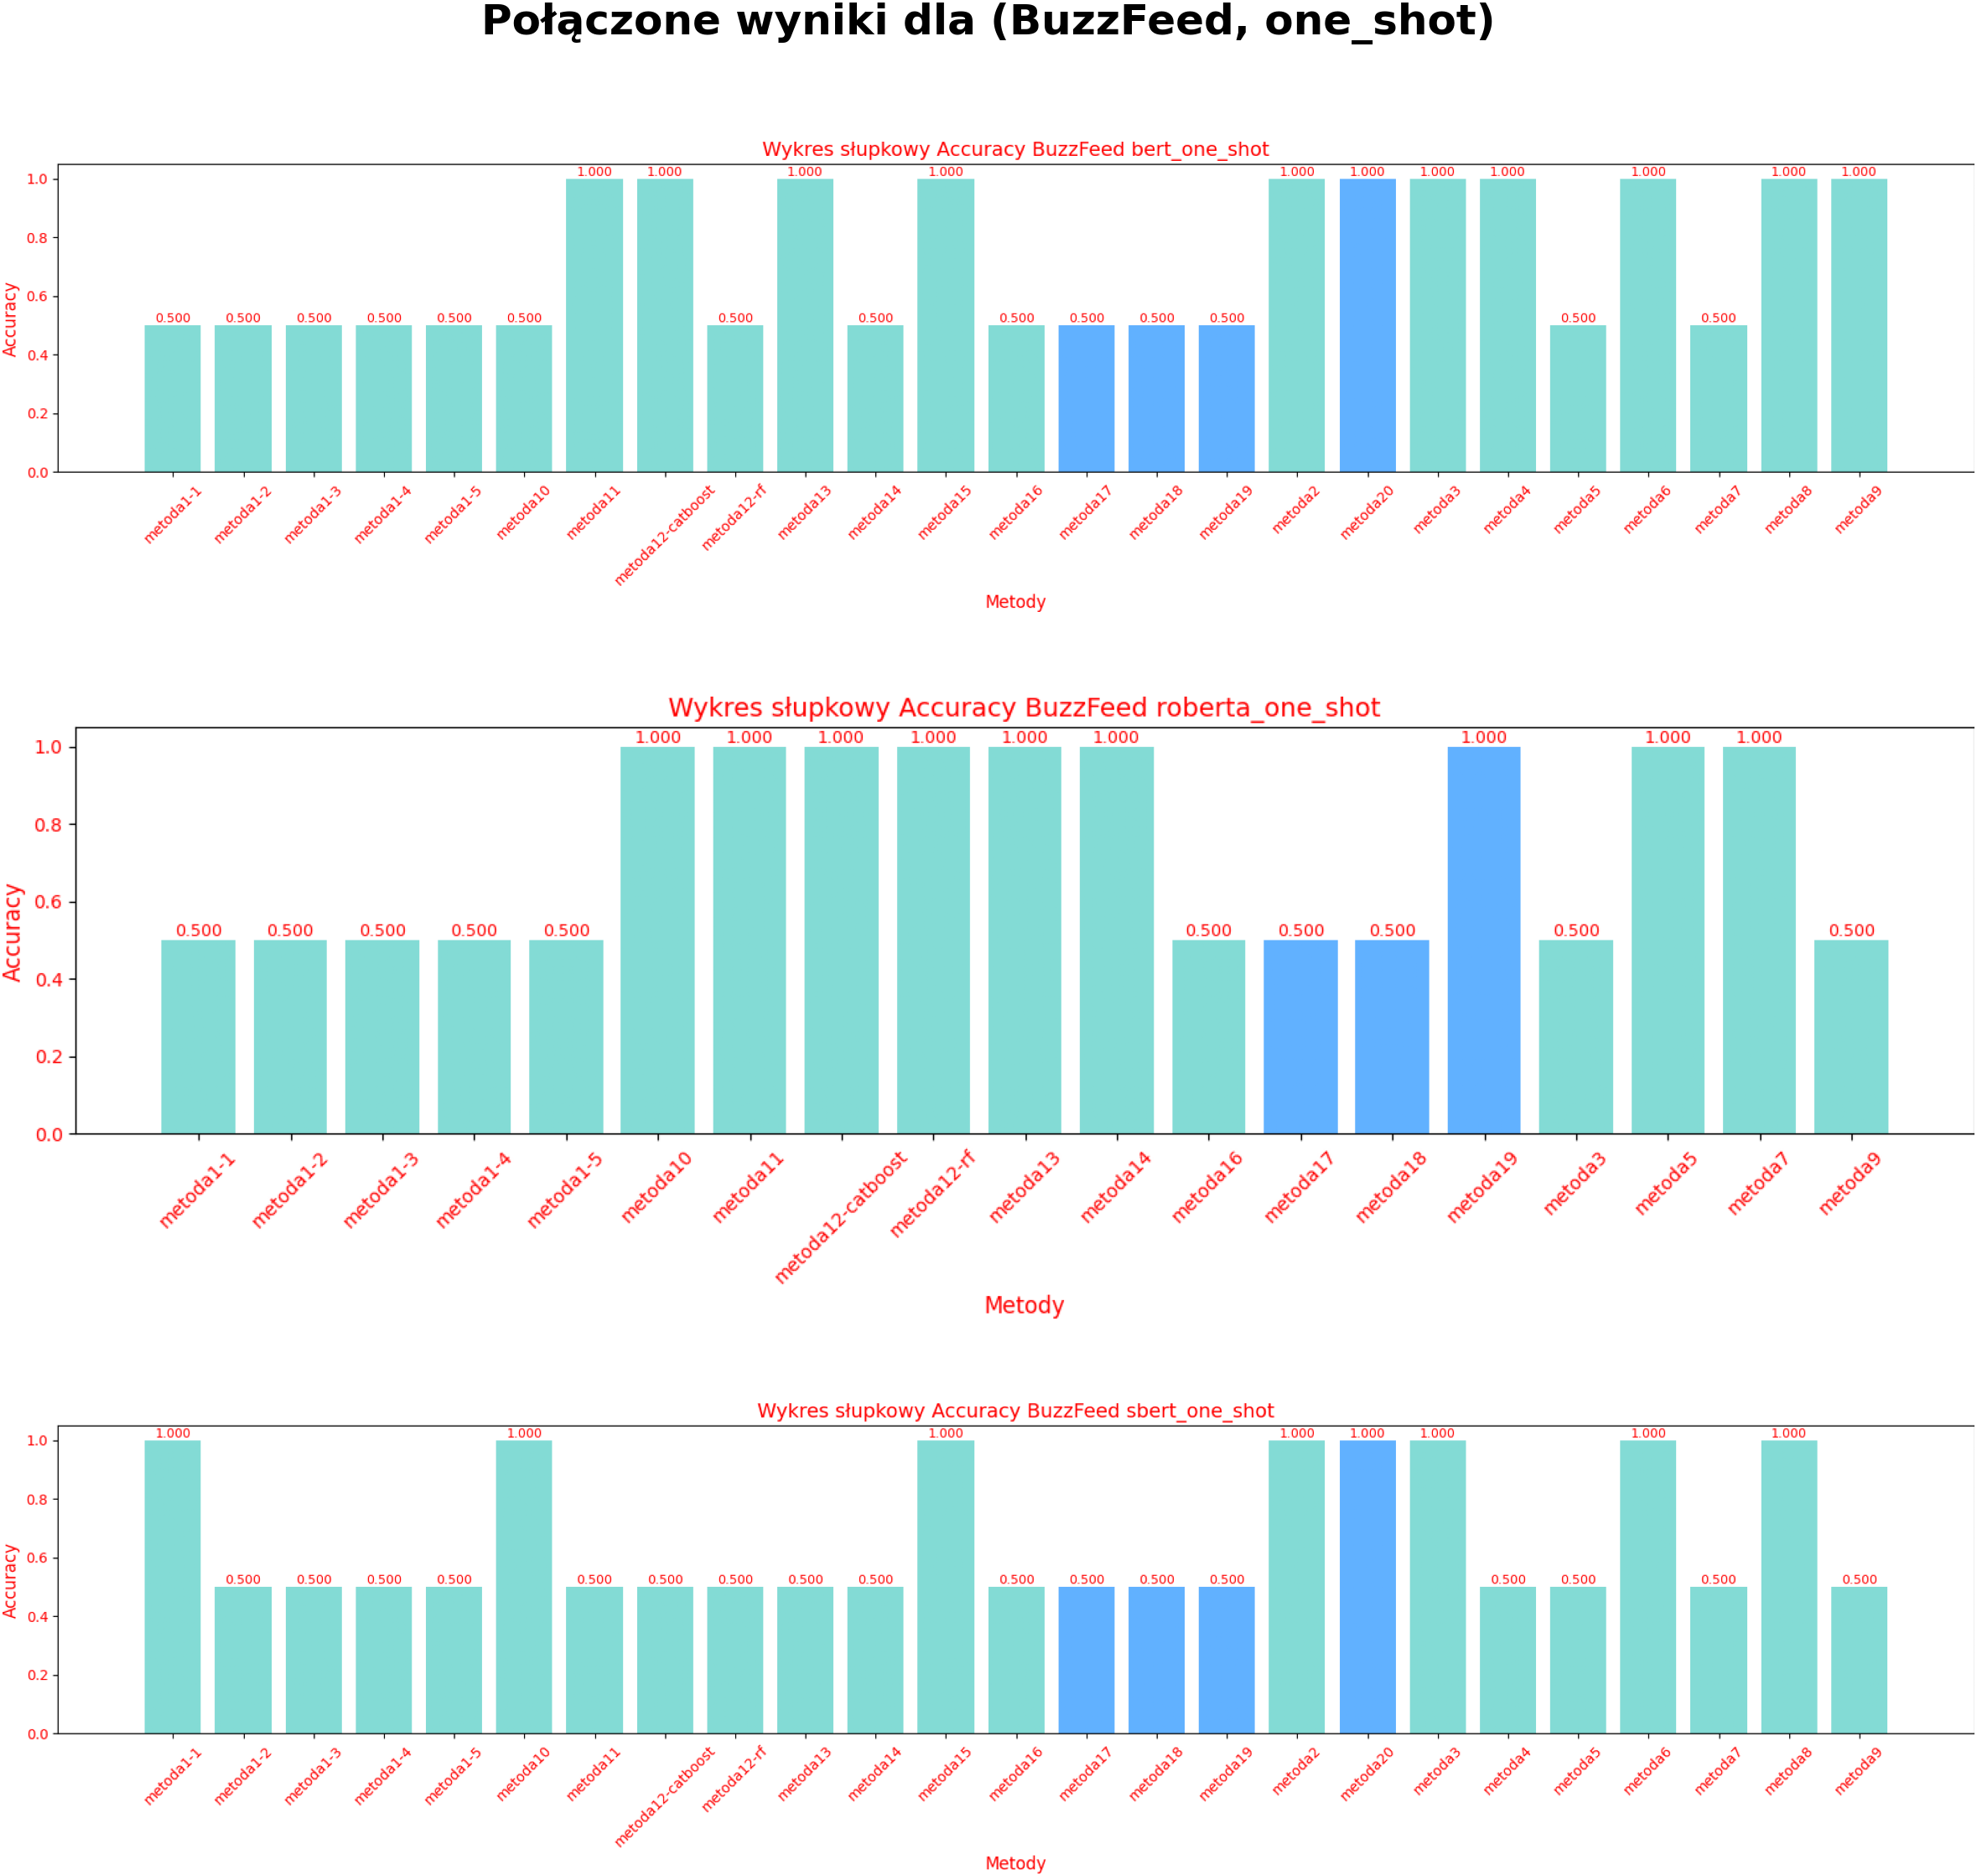
\includegraphics[width=0.99\textwidth]{img/stats/BuzzFeed_one_shot/BuzzFeed_one_shot_Combined_Accuracy_bar_chart.png}
	\caption{Histogram rozkładu \textbf{Dokładności (Accuracy)}.}
	\label{fig:buzzfeed_one_shot_accuracy}
\end{figure}

\subsubsection{F1-Score}
Wykresy F1-Score (\ref{fig:buzzfeed_one_shot_f1}) wskazują, że dla BERT \texttt{Metoda11}, \texttt{Metoda20} osiągnęły ~100\%, a \texttt{Metoda19}, \texttt{Metoda16} najniższe. Dla RoBERTa \texttt{Metoda12}, \texttt{Metoda19} miały ~100\%, a \texttt{Metoda1-4} najgorsza. Dla SBERT \texttt{Metoda1-1}, \texttt{Metoda20} osiągnęły ~100\%, a \texttt{Metoda18}, \texttt{Metoda19} najniższe. \texttt{Metoda17}, \texttt{Metoda18}, \texttt{Metoda19} słabe z powodu niedopasowania do one-shot, \texttt{Metoda20} skuteczna dzięki LightGBM.

\begin{figure}[H]
	\centering
	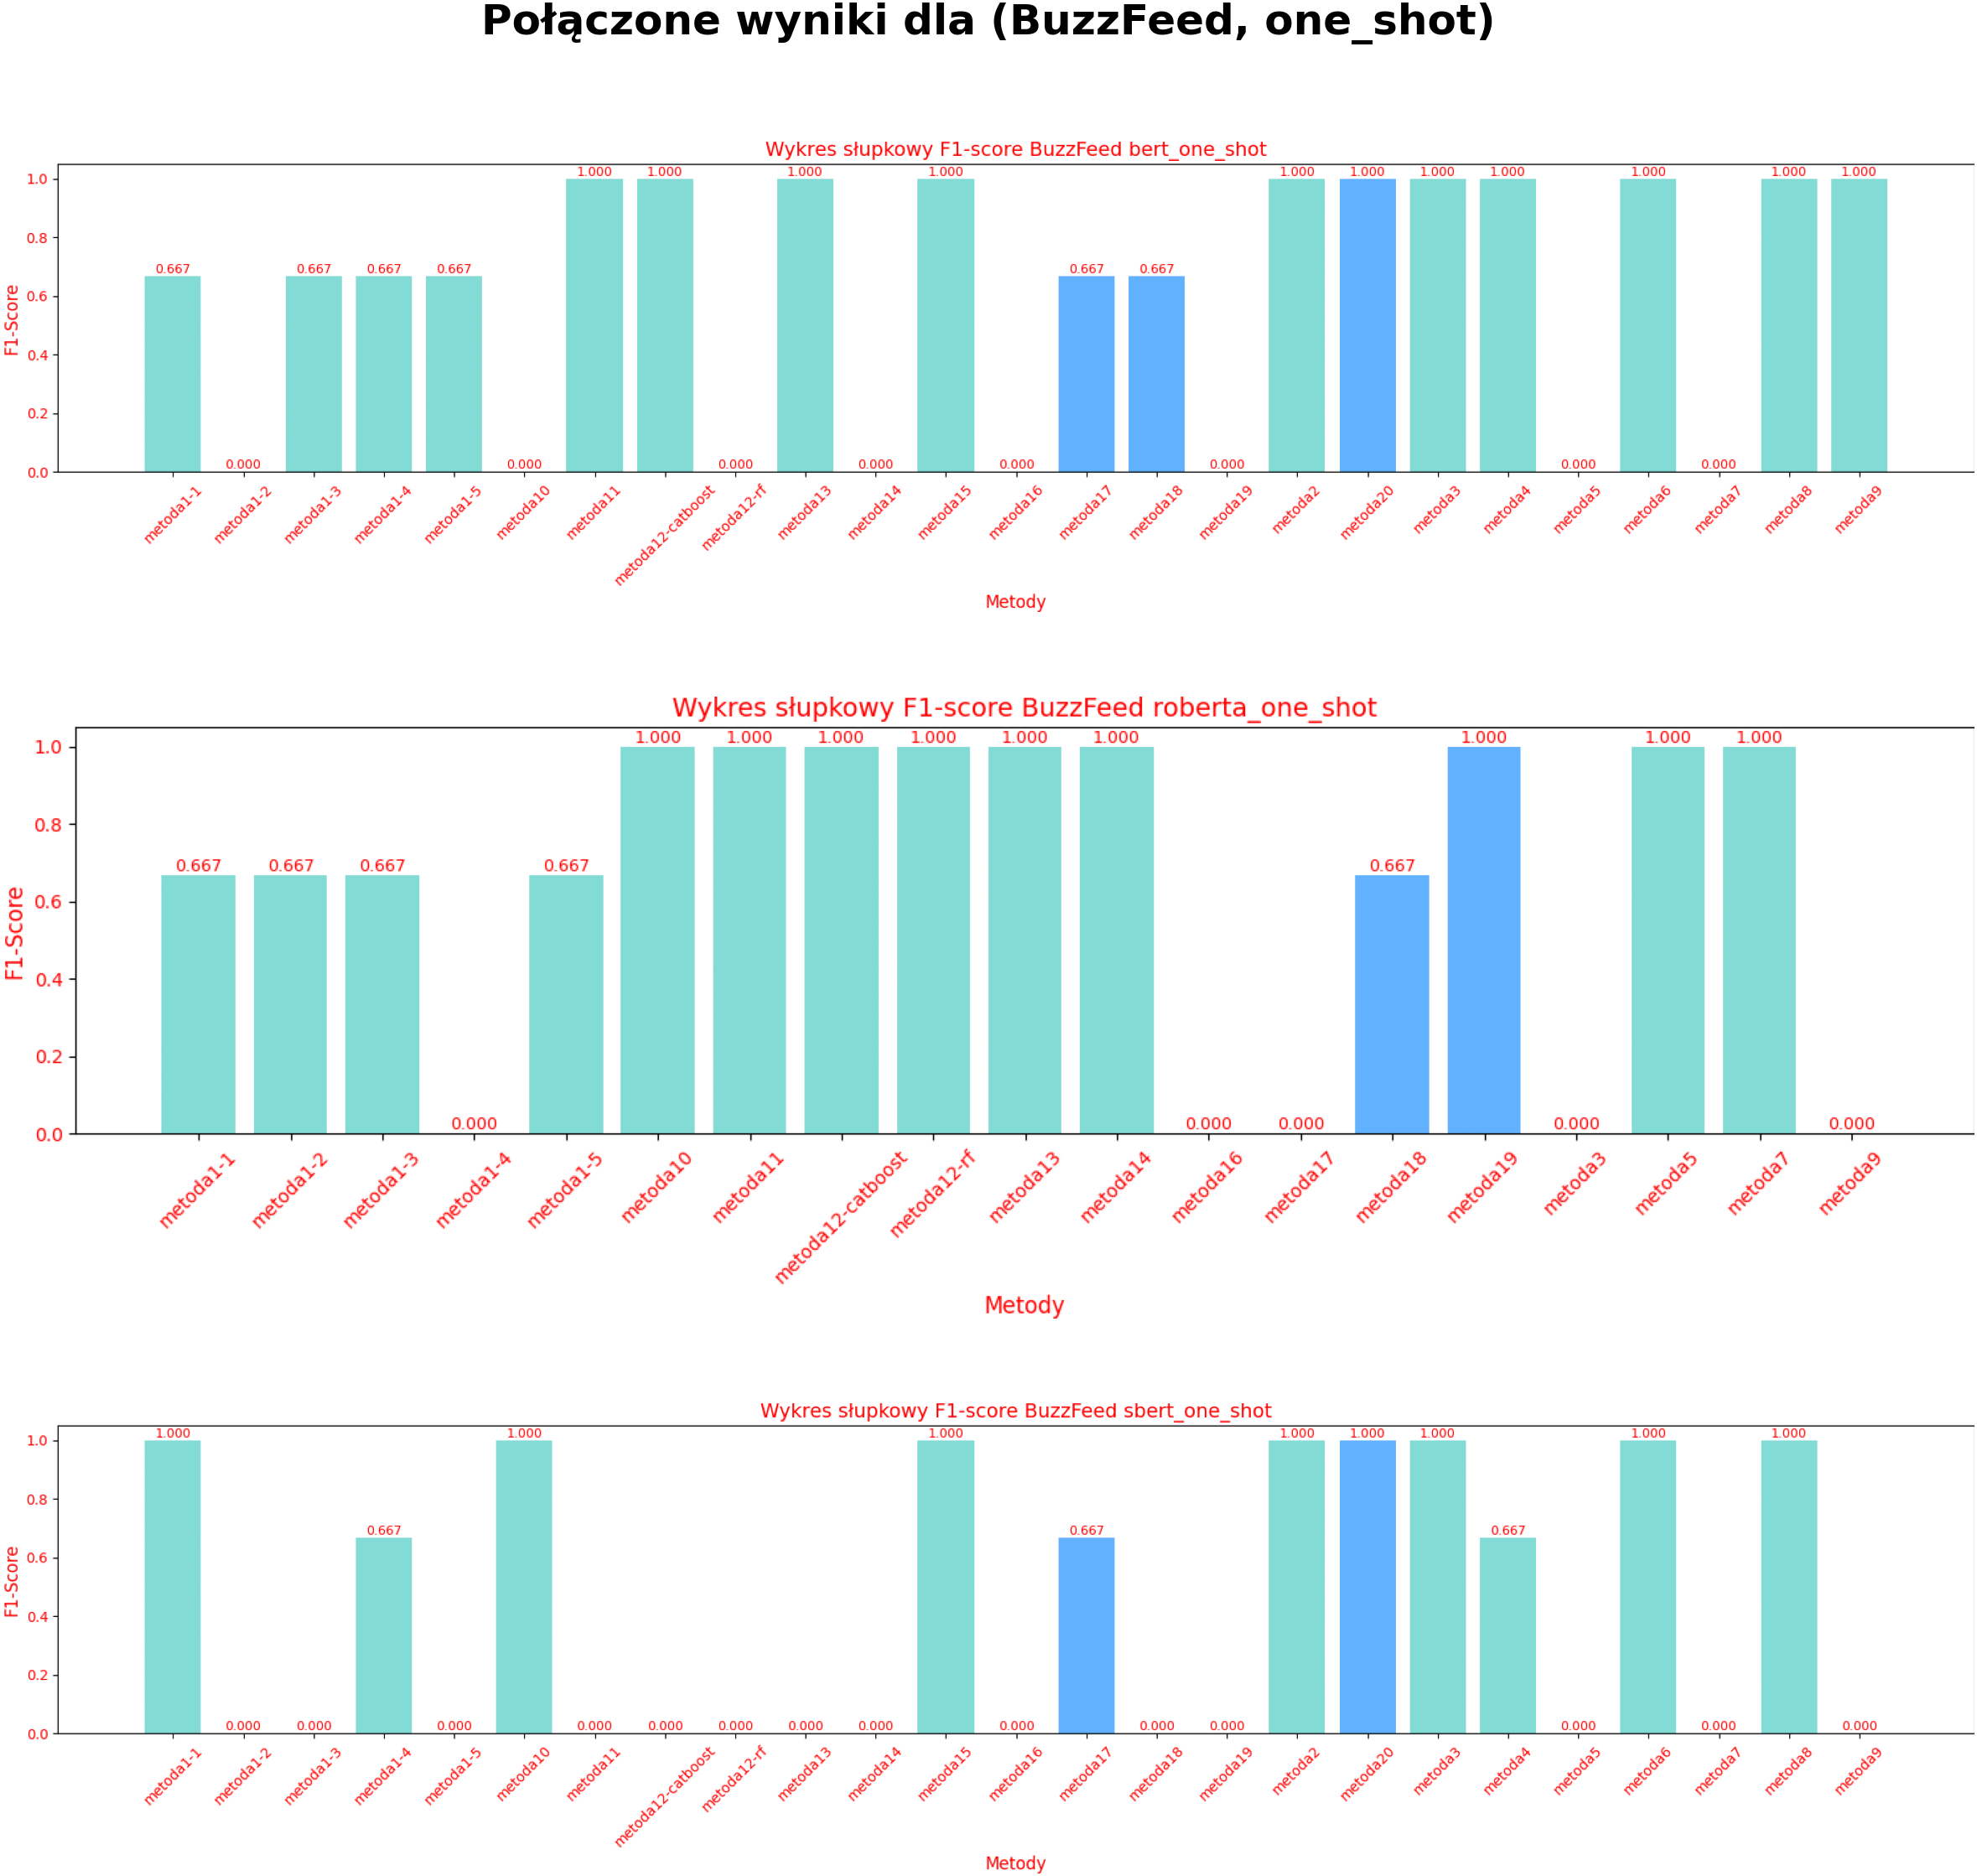
\includegraphics[width=0.99\textwidth]{img/stats/BuzzFeed_one_shot/BuzzFeed_one_shot_Combined_F1-Score_bar.png}
	\caption{Histogram rozkładu \textbf{Wyniku F1 (F1-Score)}.}
	\label{fig:buzzfeed_one_shot_f1}
\end{figure}

\subsubsection{ROC-AUC}
Wykresy ROC-AUC (\ref{fig:buzzfeed_one_shot_roc}) pokazują, że dla BERT \texttt{Metoda20}, \texttt{Metoda17} osiągnęły wysokie wyniki, a \texttt{Metoda18}, \texttt{Metoda19} najniższe. Dla RoBERTa \texttt{Metoda17}, \texttt{Metoda19} były najlepsze, a \texttt{Metoda1-x} najgorsze. Dla SBERT \texttt{Metoda20}, \texttt{Metoda11} osiągnęły wysokie wyniki, a \texttt{Metoda17}, \texttt{Metoda19} najniższe. \texttt{Metoda17} skuteczna dla RoBERTa dzięki VotingClassifier, \texttt{Metoda18} słaba dla BERT/SBERT z braku optymalizacji, \texttt{Metoda19} słaba dla SBERT z niedopasowania, \texttt{Metoda20} wysoka dzięki LightGBM.

\begin{figure}[H]
	\centering
	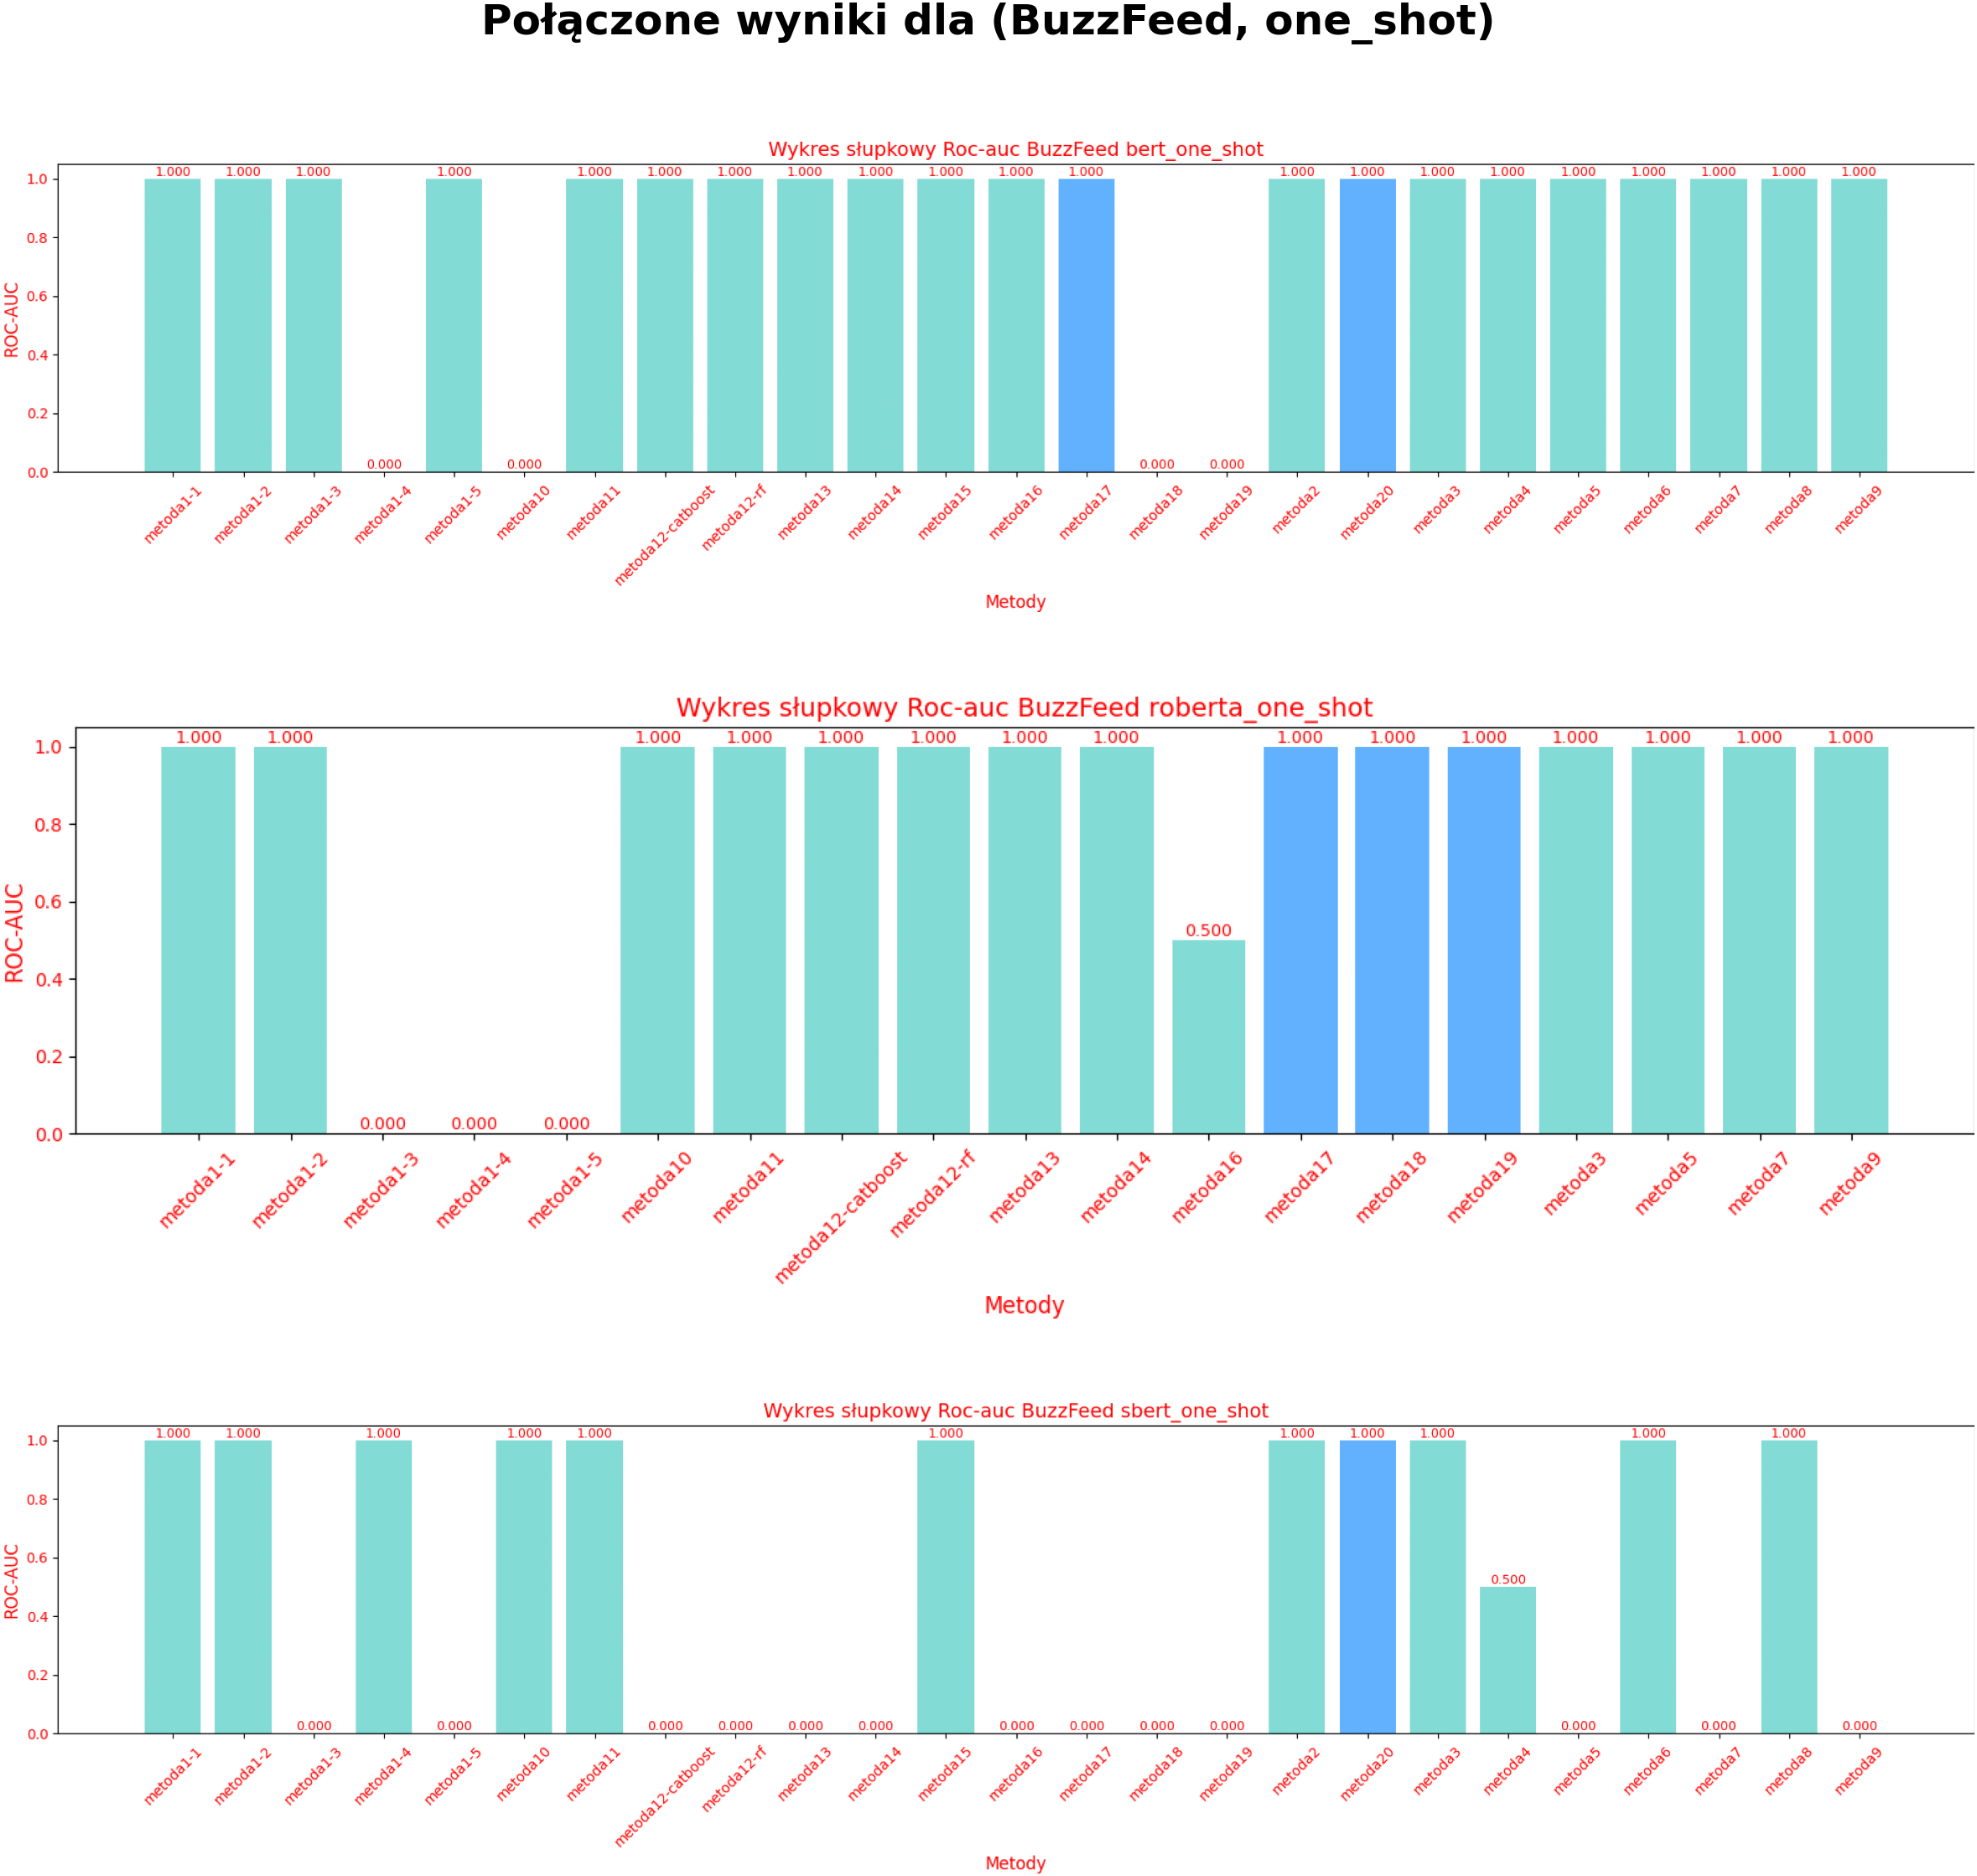
\includegraphics[width=0.99\textwidth]{img/stats/BuzzFeed_one_shot/BuzzFeed_one_shot_Combined_ROC-AUC_bar.png}
	\caption{Histogram rozkładu \textbf{Pola pod krzywą ROC-AUC (ROC-AUC)}.}
	\label{fig:buzzfeed_one_shot_roc}
\end{figure}

\subsection{Dodatkowa analiza wyników dla datasetu BuzzFeed}
\label{subsec:buzzfeed_additional_analysis}

\subsubsection{Wyniki AUC-PR}
Tabela \ref{tab:buzzfeed_auc_pr} przedstawia wyniki AUC-PR. Najwyższy wynik (0.7634) osiągnęła \texttt{metoda1-2}, a wśród metod autorskich \texttt{metoda17} (0.7041) była najlepsza. \texttt{Metoda17} skuteczna dzięki VotingClassifier, \texttt{Metoda18} (0.5893) słaba z powodu prostej konfiguracji, \texttt{Metoda19} (0.6182) średnia z braku balansowania, \texttt{Metoda20} (0.6671) dobra dzięki LightGBM.

\begin{table}[H]
	\centering
	\caption{Wyniki AUC-PR dla metod na datasecie BuzzFeed}
	\label{tab:buzzfeed_auc_pr}
	\begin{tabular}{l r}
		\toprule
		Metoda            & AUC-PR \\
		\midrule
		metoda1-1         & 0.7527 \\
		metoda1-2         & 0.7634 \\
		metoda1-3         & 0.6267 \\
		metoda1-4         & 0.6516 \\
		metoda1-5         & 0.5820 \\
		metoda2           & 0.6671 \\
		metoda3           & 0.6782 \\
		metoda4           & 0.6445 \\
		metoda5           & 0.6463 \\
		metoda6           & 0.6671 \\
		metoda7           & 0.6566 \\
		metoda8           & 0.6671 \\
		metoda9           & 0.6391 \\
		metoda10          & 0.6785 \\
		metoda11          & 0.7266 \\
		metoda12-catboost & 0.6762 \\
		metoda12-rf       & 0.6234 \\
		metoda13          & 0.6743 \\
		metoda14          & 0.6324 \\
		metoda15          & 0.6671 \\
		metoda16          & 0.6138 \\
		metoda17          & 0.7041 \\
		metoda18          & 0.5893 \\
		metoda19          & 0.6182 \\
		metoda20          & 0.6671 \\
		\bottomrule
	\end{tabular}
\end{table}

\subsubsection{Testy normalności i analizy statystyczne}
Testy Shapiro-Wilka wykazały, że większość metryk nie ma rozkładu normalnego (p-value < 0.05), z wyjątkiem ROC-AUC (p-value >= 0.05). Testy Kruskal-Wallisa nie wykazały istotnych różnic między metodami (p-value >= 0.05), co sugeruje porównywalną skuteczność.

\subsubsection{Analiza korelacji}
Macierze korelacji Pearsona i Spearmana ujawniły silne dodatnie zależności między Accuracy a Cohen's Kappa (0.9996 w Pearsonie, 0.9992 w Spearmanie), Accuracy a MCC (0.9974 w Pearsonie, 0.9907 w Spearmanie) oraz ROC-AUC a AUC-PR (0.9376 w Pearsonie, 0.9101 w Spearmanie). Brak ujemnych korelacji wskazuje na zgodność metryk.

\begin{table}[H]
	\centering
	\caption{Kluczowe współczynniki korelacji Pearsona}
	\label{tab:buzzfeed_pearson_correlations}
	\begin{tabular}{l r l}
		\toprule
		Para metryk               & Współczynnik Pearsona & Interpretacja         \\
		\midrule
		Accuracy -- Cohen's Kappa & 0.9996                & Bardzo silna dodatnia \\
		Accuracy -- MCC           & 0.9974                & Bardzo silna dodatnia \\
		MCC -- Cohen's Kappa      & 0.9977                & Bardzo silna dodatnia \\
		Precision -- F1-Score     & 0.8777                & Silna dodatnia        \\
		Recall -- F1-Score        & 0.7355                & Silna dodatnia        \\
		ROC-AUC -- AUC-PR         & 0.9376                & Bardzo silna dodatnia \\
		\bottomrule
	\end{tabular}
\end{table}

\begin{table}[H]
	\centering
	\caption{Kluczowe współczynniki korelacji Spearmana}
	\label{tab:buzzfeed_spearman_correlations}
	\begin{tabular}{l r l}
		\toprule
		Para metryk               & Współczynnik Spearmana & Interpretacja         \\
		\midrule
		Accuracy -- Cohen's Kappa & 0.9992                 & Bardzo silna dodatnia \\
		Accuracy -- MCC           & 0.9907                 & Bardzo silna dodatnia \\
		MCC -- Cohen's Kappa      & 0.9868                 & Bardzo silna dodatnia \\
		Precision -- F1-Score     & 0.8147                 & Silna dodatnia        \\
		Recall -- F1-Score        & 0.7760                 & Silna dodatnia        \\
		ROC-AUC -- AUC-PR         & 0.9101                 & Bardzo silna dodatnia \\
		\bottomrule
	\end{tabular}
\end{table}

\subsection{Podsumowanie wniosków}
Analiza wyników dla datasetu BuzzFeed pokazuje, że zaawansowane modele ensemble, takie jak \texttt{Metoda12-catboost}, \texttt{Metoda13}, \texttt{Metoda19}, \texttt{Metoda20}, osiągają wysoką skuteczność w trybach klasycznym, few-shot i one-shot, szczególnie dla embeddingów RoBERTa i SBERT. W trybie one-shot RoBERTa i SBERT umożliwiają perfekcyjne wyniki (~100\% Accuracy i F1-Score), podczas gdy BERT jest mniej skuteczny (~50\% dla wielu metod). \texttt{Metoda17} (VotingClassifier) jest skuteczna dla RoBERTa, ale słaba dla BERT z powodu niedopasowania hiperparametrów. \texttt{Metoda18} (stacking z CatBoost) dominuje dla RoBERTa w trybie few-shot, ale zawodzi dla BERT z powodu prostej konfiguracji. \texttt{Metoda19} (stacking) osiąga wysokie wyniki dla BERT/SBERT dzięki zoptymalizowanemu łączeniu modeli, ale jest słaba dla RoBERTa z braku optymalizacji. \texttt{Metoda20} (LightGBM) jest skuteczna w trybie one-shot dzięki zoptymalizowanym modelom, ale średnia w innych trybach z powodu braku balansowania klas. Prostsze modele (\texttt{Metoda1-x}) są zróżnicowane, osiągając dobre wyniki dla SBERT, ale słabsze dla BERT. Wysoka kontrastowość klas w BuzzFeed \cite{Frost2016photon} ułatwia klasyfikację dla zoptymalizowanych metod, ale wymaga precyzyjnej konfiguracji w trudniejszych scenariuszach.